\documentclass[12pt]{article}

\usepackage{sbc-template}
\usepackage{graphicx,url}
\usepackage[utf8]{inputenc}
\usepackage[brazil]{babel}
\usepackage{amsmath}
\usepackage{pdfpages}
\usepackage{realboxes}
\usepackage{array}
\usepackage{booktabs}
\usepackage{multirow}
\usepackage{float}
\usepackage{float}
\usepackage[square, numbers]{natbib} % Bibliography citation framework (in the style "[9]")
\usepackage{hyperref}
\usepackage{bookmark}
\usepackage{siunitx}
% \usepackage[numbib]{tocbibind} % number bibliography as section

\bookmarksetup{
	numbered,
	open
}

\setcitestyle{numbers}
% \usepackage[latin1]{inputenc}  



\graphicspath{ {figures/} }
% \newcommand{\PreserveBackslash}[1]{\let\temp=\\#1\let\\=\temp}
% \newcolumntype{C}[1]{>{\PreserveBackslash\centering}p{#1}}
% \newcolumntype{R}[1]{>{\PreserveBackslash\raggedleft}p{#1}}
% \newcolumntype{L}[1]{>{\PreserveBackslash\raggedright}p{#1}}
\newcolumntype{C}[1]{>{\centering\arraybackslash}p{#1}}
\newcolumntype{R}[1]{>{\raggedleft\arraybackslash}p{#1}}
\newcolumntype{L}[1]{>{\raggedright\arraybackslash}p{#1}}

\def\m#1{{\normalsize\textcircled{\scriptsize #1}}}

\sloppy
\raggedbottom

\begin{document} 


\includepdf[pages=-]{cover.pdf}

\pagenumbering{roman}
\pagestyle{empty}

\phantomsection
\addcontentsline{toc}{section}{Resumo}
\section*{Resumo}

% Uma forma encontrada por empresas desde tempos antigos a lidar com a necessidade de
% investimentos financeiros foi a abertura de capital através da venda de ações.
% Um dos exemplos mais antigos foram as \textit{commendas} na Itália Medieval, sendo que o
% primeiro estabelecimento voltado para um mercado de ações ocorreu em 1602 na Holanda.

Observação de preços em mercados sempre foi do interesse daqueles que negociavam produtos,
pois a capacidade de interpretar o mercado e decidir a melhor hora de comprar ou vender
poderia ditar a diferença entre ganhar ou perder dinheiro. Durante a Era Meiji, no Século 18,
um mercador de arroz chamado Muneshima Homma desenvolveu uma técnica de visualização e
interpretação do preço do arroz, que flutuava constantemente durante um dia de negociações.
Ele se tornou capaz de reconhecer os momentos em que o preço estaria mudando entre baixas e
altas, reconhecendo o melhor momento para negociar o produto.

% Desde então, assim como várias outras áreas tecnológicas e comerciais, os mercados se
% modernizaram com a computação. Durante esse período de modernização, em 1971 surgiu a NASDAQ:
% o primeiro mercado de ações eletrônico. Com a popularização da Internet, meios de transporte
% mais rápidos e com maior capacidade de carga, os mercados internacionais também proliferaram.
% Em paralelo ao desenvolvimento global e dos mercados, mais empresas começaram a abrir seu
% capital vendendo suas ações no mercado para investidores.

% Todo este ambiente contribuiu para que o mercado de ações se tornar uma forma atrativa de
O ambiente tecnológico atual, onde a computação e a Internet facilitaram a velocidade de
transmissão e acesso a informação contribuiu para fomentar o crescimento de 
\textit{commodities}, derivativos e opções.
Porém, com as rápidas flutuações dos preços dos ativos negociados em bolsa de valores,
causadas pelos inúmeros investidores negociando os ativos, a bolsa de valores não é um
ambiente de fácil entrada para novos investidores.
Diversos economistas e analistas se especializaram em observar, entender e predizer os
movimentos dos preços no mercado de ações através da análise fundamentalista ou gráfica
com a ajuda de indicadores derivados de preços.

Entre os especialistas em análise gráfica, em 1938 se destacou Ralph Nelson Elliott com
o seu trabalho: O Princípio das Ondas.
Sua teoria era capaz de interpretar o estado do mercado e predizer movimentos futuros com
base nos padrões das Ondas observadas. Porém, sua teoria foi considerada subjetiva por alguns
estudiosos, o que pode ter evitado a disseminação de seus estudos. Mais tarde, em 1987,
Glen Neely publicou um método científico capaz de implementar a teoria de Elliott, através
de um algoritmo que gera resultados objetivos e replicáveis.

O objetivo deste trabalho é implementar o algoritmo de Neely para análise do preço de ativos,
e analisar como diferentes configurações do método alteram a análise resultante.

\newpage

% Indexes

\phantomsection
\addcontentsline{toc}{section}{Lista de Figuras}
\listoffigures

\newpage
\phantomsection
\addcontentsline{toc}{section}{Lista de Tabelas}
\listoftables

\newpage

\phantomsection
\addcontentsline{toc}{section}{Sumário}
\tableofcontents

\newpage

\pagenumbering{arabic}
\pagestyle{plain}

\section{Introdução}
\subsection{Contextualização: Mercado Financeiro e Negociação de Ações} \label{sec:Stockmarket}

Stringham e Curott em \cite{StringhamCurott:2015} pesquisaram e descobriram que 
negócios com múltiplos acionistas se tornaram populares com contratos \textit{commenda}
na Itália Medieval \cite{Greif:2006}, e Malmendier \cite{Malmendier:2009} proveu evidências
que empresas acionistas remontam à Roma antiga. No entanto, Stringham e Curott identificaram
que o primeiro mercado de ações do mundo nasceu em Amsterdã do século 17, onde um mercado
secundário ativo de ações emergiu. As duas maiores empresas eram a Dutch East India Company
e a Dutch West India Company, fundadas em 1602 e 1621. 

Com a fundação do primeiro mercado de ações eletrônico, a NASDAQ, em 1971, e a popularização
da computação e Internet durante as últimas décadas, investir no mercado financeiro se
torna cada vez mais fácil. Porém, preços de ativos no mercado financeiro flutuam de acordo
com as negociações feitas no próprio mercado. A volatilidade deste tipo de negócio implica
que, para se obter sucesso neste tipo de empreendimento, é necessário saber observar e entender
as tendências dos preços e como eles refletem o otimismo e pessimismo dos negociadores.

\subsection{Representações Gráficas: OHLC (\textit{Open-High-Low-Close})} \label{sec:OHLC}

De acordo com a pesquisa de Lo e Hasanhodzic \cite{LoHasanhodzic:2010}, o primeiro registro
de preços com o objetivo de predizê-los ocorreu na Babilônia, durante o primeiro milênio a.C..
Segundo Shimizu \cite{Shimizu:1986} ``a abertura de trocas de \textit{commodities} na
Europa Ocidental (1561) e Japão (1654) proveram o ambiente necessário para o desenvolvimento
do gráfico''. Conforme Kirkpatrick e Dahlquist \cite{KirkpatrickDahlquist:2006},
no momento em que estas negociações aconteciam, os mercados haviam se tornado sofisticados
o bastante para produzirem múltiplos preços durante o decorrer do dia, e criando portanto,
a necessidade de se registrar os preços de abertura, máximo, mínimo e de fechamento dos
\textit{commodities} sendo negociados.

Atualmente, a forma mais comum de representar o histórico do preço de uma ação é observando
a dinâmica dos preços negociados através dos valores de abertura, máximo, mínimo, e fechamento
de um dado período.
Os quatro valores podem ser condensados em um único marcador gráfico, sendo os dois mais
comuns as ``velas japonesas'' (\textit{candelstick}), e o OHLC (\textit{Open-High-Low-Close},
literalmente Abertura-Máximo-Mínimo-Fechamento). O marcador OHLC também é conhecido como
gráfico de barras. O marcador OHLC divide seu nome com os tipos de dados de negociações de
ativos.

Os valores podem ser observados durante diferentes períodos, como um dia ou um minuto.
Na Figura \ref{fig:candlestick_chart} podem ser vistos os preços da cotação do Dólar (US\$)
em Reais (RS\$) durante o dia 5 de Fevereiro de 2018, utilizando as marcações de
\textit{candlesticks} com intervalos de tempo de 1 hora.

\begin{figure}[H]
	\centering
	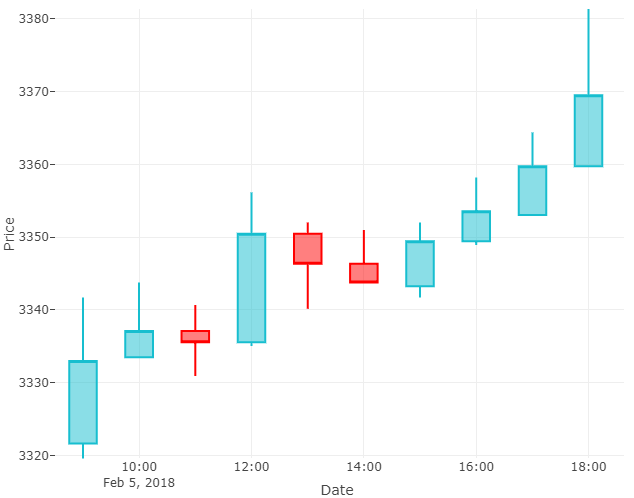
\includegraphics[width=0.8\textwidth]{candlestick_chart.png}
	\caption{Gráfico do Preço do Dólar (2018-02-05) em \textit{candlesticks}}
	\label{fig:candlestick_chart}
\end{figure}

Cada ``vela'' representa um conjunto de quatro valores: abertura (\textit{open}),
máximo (\textit{high}), mínimo (\textit{low}) e fechamento (\textit{close}).
A extensão do ``pavio'' da vela indica os valores de máximo (extensão superior) e mínimo
(extensão inferior), e os valores de abertura e fechamento são indicados pelo ``corpo''
da vela.
Os preços observados as 12:00 e 13:00 podem ser vistos na Figura \ref{fig:chart_dynamic}.

\begin{figure}[H]
	\centering
	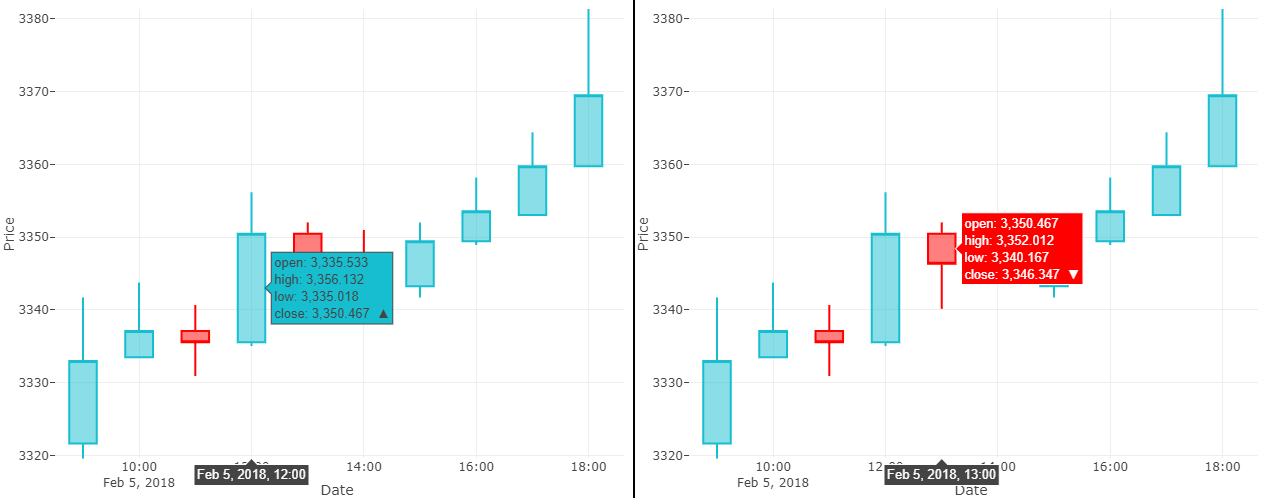
\includegraphics[width=\textwidth]{chart_dynamic.png}
	\caption{Preço do Dólar (2018-02-05) as 12:00 e 13:00}
	\label{fig:chart_dynamic}
\end{figure}

É notável observar que as 12:00 o preço aumenta durante o período (preço de fechamento é
maior que o preço de abertura), enquanto as 13:00 ocorre o contrário (preço de fechamento é
menor  que o preço de abertura). Preços crescentes e decrescentes são distinguidos por cores
(e.g. azul para crescente, vermelho para decrescente) ou por vela sem cor interna (crescente)
ou com cor cheia (decrescente) em representações monocromáticas. Essa distinção é necessária,
caso contrário não é possível observar no corpo da vela se o preço de abertura/fechamento
ocorreu no topo ou na base do corpo da vela.

O mesmo histórico de preço mostrado na Figura \ref{fig:candlestick_chart}
pode ser visto na Figura \ref{fig:ohlc_chart} a seguir utilizando marcadores OHLC.

\begin{figure}[H]
	\centering
	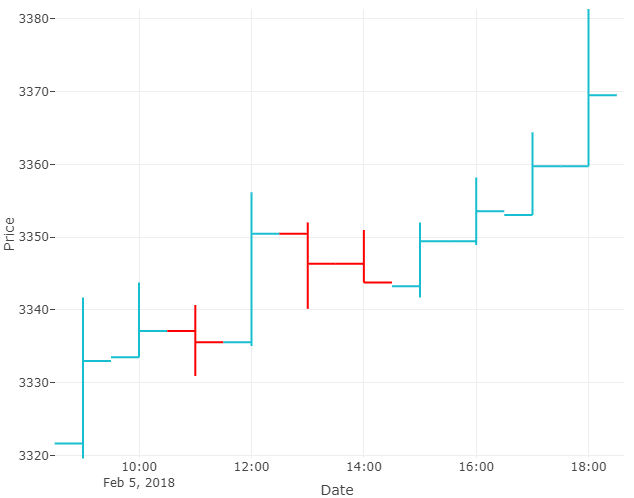
\includegraphics[width=0.8\textwidth]{ohlc_chart.png}
	\caption{Gráfico do Preço do Dólar (2018-02-05) em OHLC}
	\label{fig:ohlc_chart}
\end{figure}

Na representação OHLC, o traço vertical indica os valores de máximo e mínimo, a extensão
a esquerda indica o valor de abertura, e a extensão a direita indica o valor de fechamento.
Em contrapartida às \textit{candlesticks} não é necessário uma representação em cores para
distinguir abertura de fechamento no indicador, porém, a visualização toma menos volume no
gráfico, o que pode dificultar a leitura ao observador.

Os dois marcadores podem ser vistos lado a lado na Figura \ref{fig:chart_comp} para efeito
de comparação.

\begin{figure}[H]
	\centering
	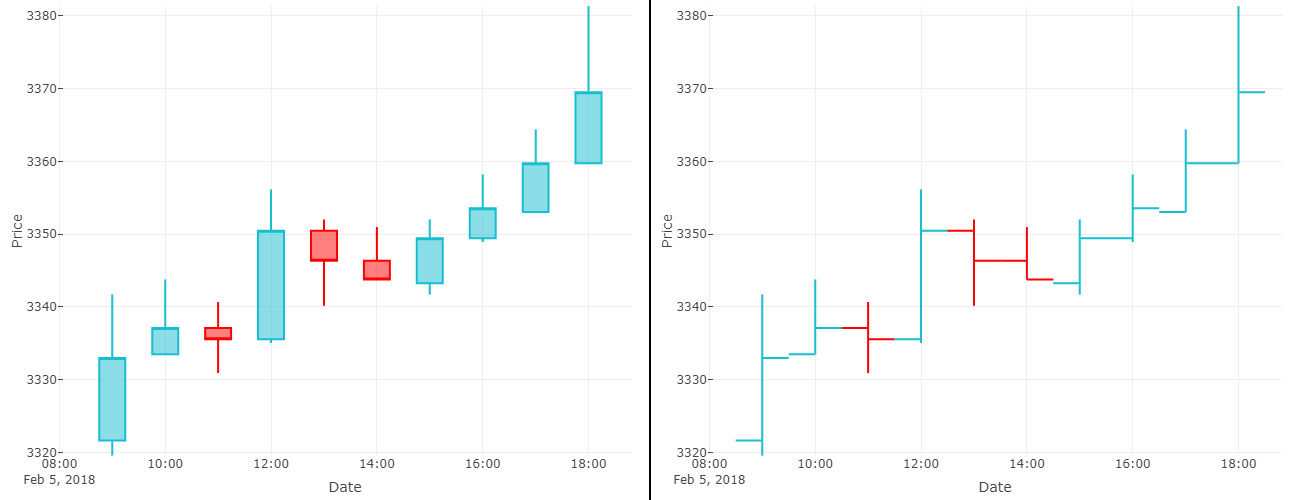
\includegraphics[width=\textwidth]{chart_comp.png}
	\caption{Gráfico do Preço do Dólar (2018-02-05)}
	\label{fig:chart_comp}
\end{figure}

É importante ressaltar também que gráficos de preços de ativos procuram representar a dinâmica 
do preço durante um período, já que o preço de um ativo muda constantemente. Os preços do Dólar
observados na Figura \ref{fig:ohlc_chart} representam um período de 1 hora para cada ponto
no gráfico. Os valores do Dólar para o mesmo dia, porém com período de 1 minuto, podem ser
observados na Figura \ref{fig:ohlc_chart_detailed} a seguir.

\begin{figure}[H]
	\centering
	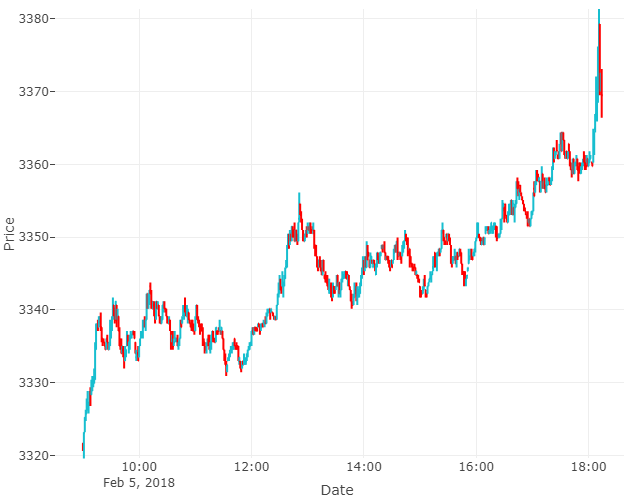
\includegraphics[width=0.8\textwidth]{ohlc_chart_detailed.png}
	\caption{Gráfico do Preço do Dólar (2018-02-05) com maior Resolução}
	\label{fig:ohlc_chart_detailed}
\end{figure}

Apesar de serem observados os mesmos preços no mesmo dia, a resolução pode mudar completamente
a interpretação do gráfico. Uma comparação superimposta da Figura \ref{fig:candlestick_chart}
e da Figura \ref{fig:ohlc_chart_detailed} pode ser vista na
Figura \ref{fig:ohlc_chart_detailed_superimposed} a seguir.

\begin{figure}[H]
	\centering
	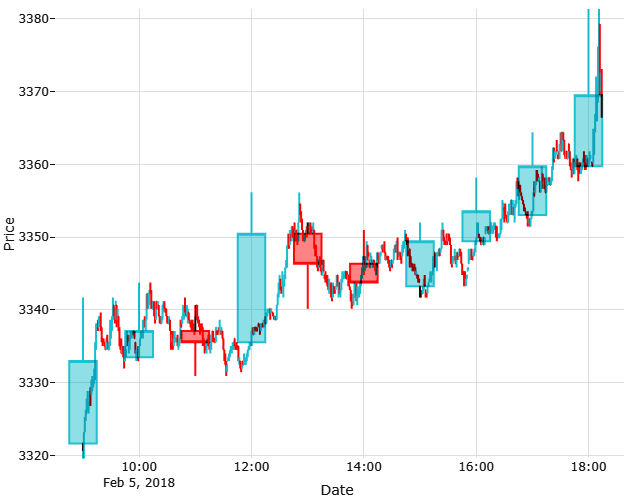
\includegraphics[width=0.8\textwidth]{ohlc_chart_detailed_superimposed.png}
	\caption{Gráfico do Preço do Dólar (2018-02-05) comparando resoluções}
	\label{fig:ohlc_chart_detailed_superimposed}
\end{figure}

Os preços do Dólar utilizados nos gráficos desta seção podem ser vistos na
Tabela \ref{tab:prices_table} a seguir. Estes preços foram exportados do programa
MetaTrader 5. Os gráficos desta seção foram gerados utilizando o programa em
desenvolvimento neste projeto de pesquisa.

\begin{table}[H]
	\centering
	\caption{Preços do Dólar (2018-02-05) em Tabela}
	\label{tab:prices_table}
	\begin{tabular}{l c c c c}
		\textbf{Data} & \textbf{Abertura} & \textbf{Máximo} & \textbf{Mínimo} & \textbf{Fechamento} \\
		\toprule
		2018/02/05 9:00 & 3,321628 & 3,341712 & 3,319568 & 3,332958\\
		\midrule
		2018/02/05 10:00 & 3,333473 & 3,343772 & 3,333473 & 3,337078\\
		\midrule
		2018/02/05 11:00 & 3,337078 & 3,340682 & 3,330898 & 3,335533\\
		\midrule
		2018/02/05 12:00 & 3,335533 & 3,356132 & 3,335018 & 3,350467\\
		\midrule
		2018/02/05 13:00 & 3,350467 & 3,352012 & 3,340167 & 3,346347\\
		\midrule
		2018/02/05 14:00 & 3,346347 & 3,350982 & 3,343772 & 3,343772\\
		\midrule
		2018/02/05 15:00 & 3,343257 & 3,352012 & 3,341712 & 3,349437\\
		\midrule
		2018/02/05 16:00 & 3,349437 & 3,358192 & 3,348922 & 3,353557\\
		\midrule
		2018/02/05 17:00 & 3,353042 & 3,364372 & 3,353042 & 3,359737\\
		\midrule
		2018/02/05 18:00 & 3,353042 & 3,381366 & 3,353042 & 3,369521
	\end{tabular}
\end{table}

\newpage

\section{Análise Gráfica}
\subsection{Ondas de Elliott} \label{sec:Elliott-Waves}

% Como a análise dos preços no mercado de ações é uma maneira de se conhecer o estado
% do mercado e reconhecer momentos oportunos para investimentos, diversos especialistas
% financeiros se dedicaram a estudar os movimentos dos preços. Charles J. Collins, da
% Investment Counsel, Inc., citou no prefácio de \cite{PrechterFrost:2005} 4 especialistas
% nos estudos do comportamento do mercado: Arthur Cecil Pigou, Charles Henry Dow,
% Bernard Mannes Baruch e Ralph Nelson Elliott.

% Arthur Cecil Pigou afirmou que ``movimentos de preços (para cima ou para baixo)
% no mercado são causados por excesso de otimismo seguidos de excessos de pessimismo''.
% Charles Henry Dow (co-fundador da Dow Jones \& Company) observou que aumentos de preços
% são caracterizados por três oscilações. Bernard Mannes Baruch afirmou que ``eventos em si
% não registram flutuações no mercado de ações; o que registra as flutuações no mercado de
% ações são as reações humanas aos eventos''.

% Ralph Nelson Elliott iniciou seu estudo no início da década de 30, observando os índices
% históricos da Dow Jones. Após a recessão de da década de 29, Elliott realizou uma previsão
% do momento exato em que o mercado iria virar e romper o máximo da década de 35 e que o
% mercado  seguiria um forte movimento otimista, seguido de outra forte recessão.
% O índice Dow Jones pode ser visto durante o período de 1932 até 1938 na Figura
% \ref{fig:DowJones_history}, obtido em \cite{DowJonesHistory}.

% \begin{figure}[H]
% 	\centering
% 	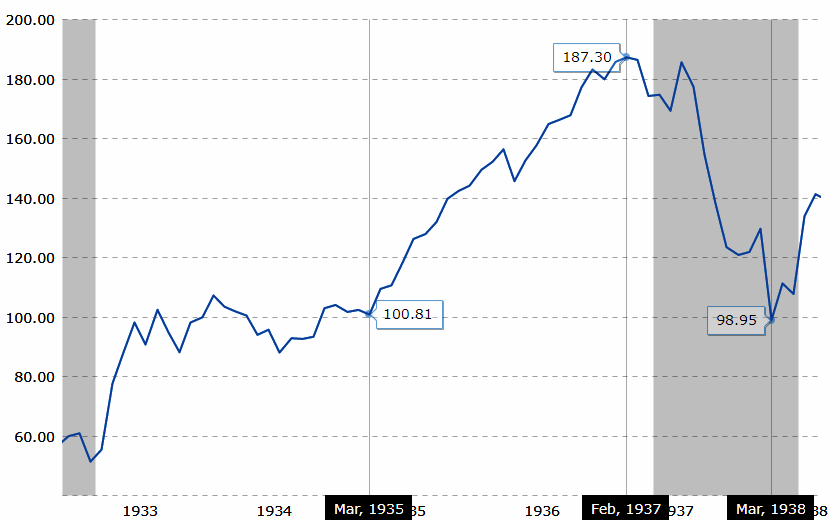
\includegraphics[width=\textwidth]{DowJones_history.png}
% 	\caption{Histórico do Índice Dow Jones 1932-1938}\label{fig:DowJones_history}
% \end{figure}

A Teoria das Ondas de Elliott pode ser explicada em alguns princípios baseados nos fenômenos
que ele observou nos preços. Estes princípios são:

\begin{itemize}
	\item Preços no mercado de ações seguem padrões reconhecíveis;
	\item Estes padrões se repetem em ``forma'', mas não necessariamente em
		  ``amplitude'' e ``tempo'';
	\item Estes padrões são chamados de \textbf{Ondas} (\textbf{\emph{Waves}});
	\item Uma onda pode ser classificada como sendo \textbf{Motivadora}/\textbf{Motriz}
		  ou \textbf{Corretiva};
	\begin{itemize}
		\item Ondas \textbf{Motivadoras} (\textbf{\emph{Motive}}) seguem a
			  \textbf{mesma tendência} do mercado;
		\item Ondas \textbf{Corretiva} (\textbf{\emph{Corrective}}) seguem a
			  \textbf{tendência contrária} a do mercado;
	\end{itemize}
	\item As \textbf{Ondas} podem ser combinadas entre si para formarem \textbf{novas Ondas}
		  em \textbf{resoluções de tempo} diferentes (visão fractal);
\end{itemize}

A onda idealizada observada por Elliott foi o padrão de Onda 5-3, visto na Figura
\ref{fig:ElliottWave5-3}.
As Ondas de Elliott motivadoras são identificadas com números e as corretivas são
identificadas com letras.

\begin{figure}[H]
	\centering
	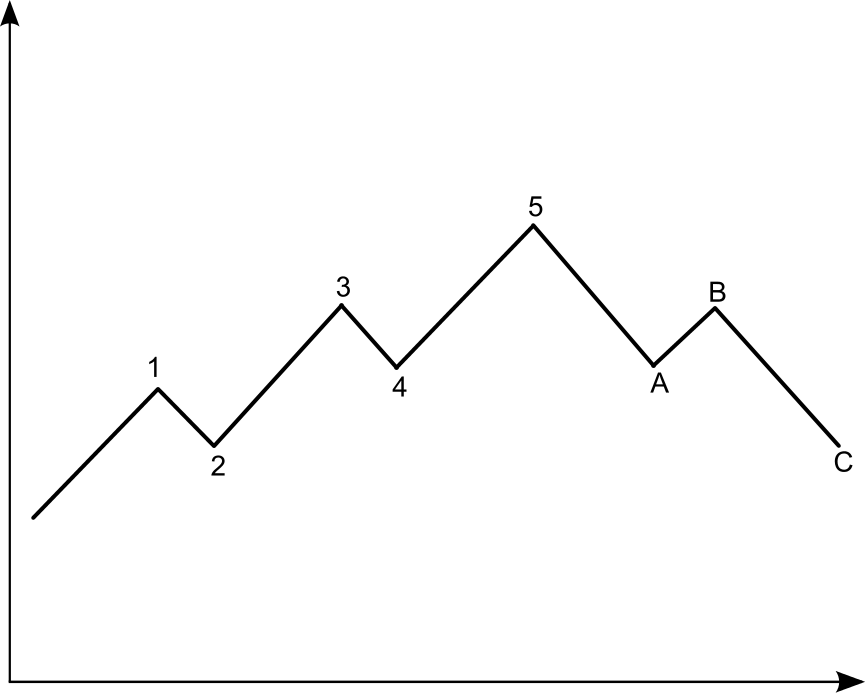
\includegraphics[width=0.7\textwidth]{ElliottWave5-3.png}
	\caption{Onda Padrão 5-3 (adaptado de \cite{Masur})}\label{fig:ElliottWave5-3}
\end{figure}

A tendência principal do mercado é que um Impulso (Onda 1-2-3-4-5 na
Figura \ref{fig:ElliottWave5-3}) sempre é seguido de uma Retração (Onda A-B-C), formando o
padrão 5-3, onde há 5 Ondas para o impulso e 3 Ondas para a retração.
Adicionalmente, como as Ondas podem ser combinadas entre si para formarem novas Ondas,
o padrão de ondas 5-3 também poderia ser observado como na Figura
\ref{fig:ElliottWave5-3_extended}.

\begin{figure}[H]
	\centering
	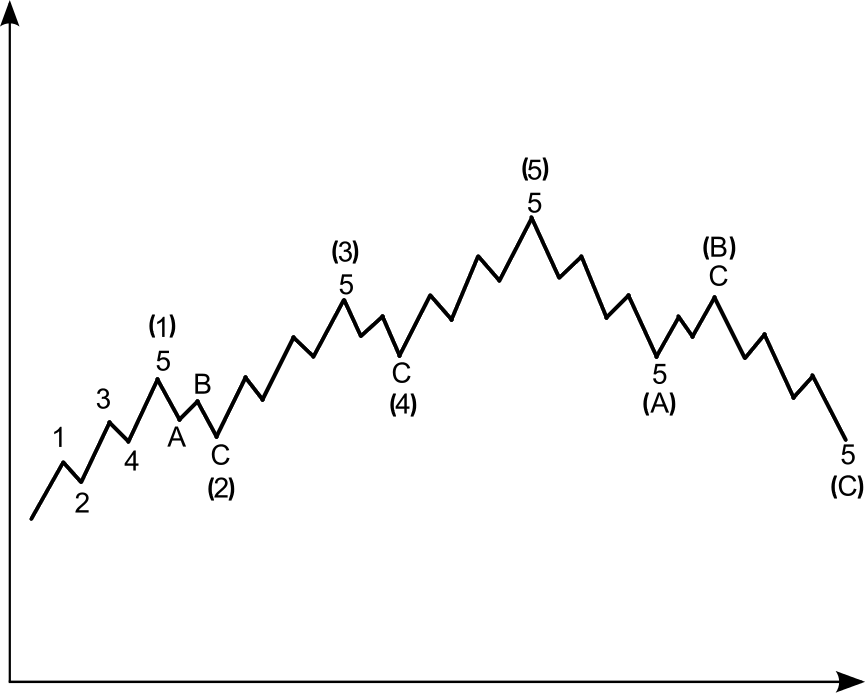
\includegraphics[width=0.7\textwidth]{ElliottWave5-3_extended.png}
	\caption{Onda Padrão 5-3 estendida (adaptado de \cite{Masur})}
	\label{fig:ElliottWave5-3_extended}
\end{figure}

Quando um conjunto de Ondas forma uma nova onda em uma resolução de tempo diferente, é dito que
as Ondas formam uma onda de grau superior. Dessa forma, se torna necessária uma regra de
identificação para Ondas de acordo com o grau (resolução do tempo) na qual elas se encontram.
As marcações utilizadas para cada grau podem ser vistas na
Tabela \ref{tab:ElliottWaveDegreeNotations} a seguir. Os ``5's Seguindo a Tendência'' são
como são identificadas as ondas motivadoras (usando números), e os
``3's Contra a Tendência'' são como são identificadas as ondas corretivas (usando letras).

\begingroup
\scriptsize
\begin{table}[H]
	\centering
	\caption{Notações das Ondas de Elliott de acordo com o Grau da Onda}
	\label{tab:ElliottWaveDegreeNotations}
\begin{tabular}{rlccccccccc}
   & \multicolumn{1}{l}{Grau da Onda} & \multicolumn{5}{c}{5's Seguindo a} &  & \multicolumn{3}{c}{3's Contra a} \\
   & \multicolumn{1}{c}{} & \multicolumn{5}{c}{Tendência} &  & \multicolumn{3}{c}{Tendência} \\
\toprule
 1 & Supermilênio		& \m{1}	& \m{2}	& \m{3}	& \m{4}	& \m{5}	& & \m{A} & \m{B} & \m{C} \\
 2 & Milênio			& (1)	& (2)	& (3)	& (4)	& (5)	& & (A)	  & (B)	  & (C)	  \\
 3 & Submilênio			& 1		& 2		& 3		& 4		& 5		& & A	  & B	  & C	  \\
\midrule
 4 & SuperCiclo Maior	& \m{I}	&\m{II}	&\m{III}&\m{IV}	& \m{V}	& & \m{a} & \m{b} & \m{c} \\
 5 & SuperCiclo			& (I)	& (II)	& (III)	& (IV)	& (V)	& & (a)	  & (b)	  & (c)	  \\
 6 & Ciclo				& I		& II	& III	& IV	& V		& & a	  & b	  & c	  \\
\midrule
 7 & Primário			& \m{1}	& \m{2}	& \m{3}	& \m{4}	& \m{5}	& & \m{A} & \m{B} & \m{C} \\
 8 & Intermediário		& (1)	& (2)	& (3)	& (4)	& (5)	& & (A)	  & (B)	  & (C)	  \\
 9 & Menor				& 1		& 2		& 3		& 4		& 5		& & A	  & B	  & C	  \\
\midrule
10 & Minuto				& \m{i}	&\m{ii}	&\m{iii}&\m{iv}	& \m{v}	& & \m{a} & \m{b} & \m{c} \\
11 & Minuete			& (i)	& (ii)	& (iii)	& (iv)	& (v)	& & (a)	  & (b)	  & (c)	  \\
12 & SubMinuete			& i		& ii	& iii	& iv	& v		& & a	  & b	  & c	  \\
\midrule
13 & Micro				& \m{1}	& \m{2}	& \m{3}	& \m{4}	& \m{5}	& & \m{A} & \m{B} & \m{C} \\
14 & Submicro			& (1)	& (2)	& (3)	& (4)	& (5)	& & (A)	  & (B)	  & (C)	  \\
15 & Minúsculo			& 1		& 2		& 3		& 4		& 5		& & A	  & B	  & C	  \\
\end{tabular}
\end{table}
\endgroup

Os padrões identificados por Elliott podem ser vistos na Tabela \ref{tab:ElliottWavePatterns},
onde cada padrão pode ser visto na Figura de referência no Apêndice \ref{app:EWPatterns}.
As regras para formação de cada padrão podem ser vistas na Seção \ref{sec:ElliottWaveRuleset}
a seguir.

\begingroup
\begin{table}[H]
	\small
	\centering
	\caption{Padrões das Ondas de Elliott}
	\label{tab:ElliottWavePatterns}
\begin{tabular}{c C{5cm} C{5cm} L{2.5cm}}
	& \textbf{Padrão} & \textbf{Nome Original} & \textbf{Referência}\\
	\toprule
	\multirow{4}{*}{\rotatebox{90}{\centering\parbox{2cm}{\scriptsize\centering\textbf{Ondas\\Motivadoras}}}}
		& Impulso & \textit{Impulse} & Figura \ref{fig:EW_pattern_01} \\
		& Extensão & \textit{Extension} & Figura \ref{fig:EW_pattern_02} \\
		& Truncagem & \textit{Truncation} & Figura \ref{fig:EW_pattern_03} \\
		& Diagonal Final/Inicial & \textit{Ending/Leading Diagonal} & Figura \ref{fig:EW_pattern_04}\\
	\midrule
	\multirow{7}{*}{\rotatebox{90}{\centering\parbox{2cm}{\scriptsize\centering\textbf{Ondas\\Corretivas}}}}
		& Zigzag & \textit{Zigzag} & Figura \ref{fig:EW_pattern_05}\\
		& Zigzag Duplo & \textit{Double Zigzag} & Figura \ref{fig:EW_pattern_06}\\
		& Plano & \textit{Flat} & Figura \ref{fig:EW_pattern_07}\\
		& Plano Estendido & \textit{Extended Flat} & Figura \ref{fig:EW_pattern_08}\\
		& Plano Corrido & \textit{Running Flat} & Figura \ref{fig:EW_pattern_09}\\
		& Triângulo & \textit{Triangle} & Figura \ref{fig:EW_pattern_10}\\
		& Combinação (3 Duplo e Triplo) & \textit{Double/Triple 3} & Figuras \ref{fig:EW_pattern_11} e \ref{fig:EW_pattern_12}
\end{tabular}
\end{table}
\endgroup

\subsubsection{Regras para Formação das Ondas de Elliott}\label{sec:ElliottWaveRuleset}

\begin{itemize}
	\item Impulso
	\begin{itemize}
		\item O Impulso sempre se divide em 5 ondas
		\item Onda 2 nunca se move além do início da Onda 1
		\item Onda 3 sempre se move além do final da Onda 1
		\item Onda 4 nunca se move além do fim da Onda 1
		\item Nunca todas as Ondas 1, 3 e 5 estão todas Estendidas
		\item Onda 1 sempre subdivide em Impulso ou (raramente) Diagonal
		\item Onda 3 sempre subdivide em Impulso
		\item Onda 5 sempre subdivide em Impulso ou Diagonal
		\item Onda 2 sempre subdivide em Zigzag
		\item Onda 4 sempre subdivide em Zigzag, Triângulo ou Combinação
	\end{itemize}
	\item Diagonal
	\begin{itemize}
		\item A Diagonal sempre se subdivide em 5 Ondas
		\item A Diagonal Final sempre é a onda 5 de um Impulso, ou Onda C de um Zigzag ou Plano
		\item A Diagonal Inicial sempre aparece como Onda 1 de um Impulso ou Onda A de um Zigzag
		\item Ondas 1, 2, 3, 4, e 5 de uma Diagonal Final, e Ondas 2 e 4 de uma Diagonal Inicial, sempre se subdividem em Zigzags
		\item Onda 2 nunca passa do início da Onda 1
		\item Onda 3 sempre passa do fim da Onda 1
		\item Onda 4 nunca passa do final da Onda 2
		\item Onda 4 sempre termina dentro do território de preço da Onda 1
		\item Em relação ao tempo, uma linha conectando o fim das Ondas 2 e 4 convergem em direção (caso de contração) ou divergem (caso de expansão) de uma linha conectando os fins das Ondas 1 e 3
		\item A Onda 5 de uma Diagonal Inicial sempre termina além do final da Onda 3
		\item Na Diagonal com Contração, a Onda 3 é sempre mais curta que a Onda 1, e a Onda 5 é sempre mais curta que a Onda 3
		\item Na Diagonal com Expansão, a Onda 3 é sempre mais longa que a Onda 1, e a Onda 5 é sempre mais longa que a Onda 3			
	\end{itemize}
	\item Zigzag
	\begin{itemize}
		\item A Zigzag sempre se subdivide em 3 Ondas
		\item A Onda A sempre se subdivide em um Impulso ou em uma Diagonal Inicial
		\item A Onda C sempre se subdivide em um Impulso ou em uma Diagonal
		\item A Onda B sempre se subdivide em um Zigzag, Plano, Triângulo ou Combinação destes
		\item A Onda B nunca se move além do início da Onda A
	\end{itemize}
	\item Plano
	\begin{itemize}
		\item Um Plano sempre se subdivide em 3 Ondas
		\item Onda A nunca é um Triângulo
		\item Onda C sempre é um Impulso ou um Triângulo
		\item Onda B sempre regride/retraça pelo menos 90\% da Onda A
	\end{itemize}
	\item Triângulo
	\begin{itemize}
		\item Contracionado
		\begin{itemize}
			\item Um Triângulo sempre se subdivide em 5 Ondas
			\item Pelo menos 4 ondas entre A, B, C, D e E se subdividem em um Zigzag ou Combinação de Zigzags
			\item A Onda C nunca se move além do final da Onda A
			\item A Onda D nunca se move além do final da Onda B
			\item A Onda E nunca se move além do final da Onda C
			\item Consequência das 3 regras anteriores: uma linha ligando os fins das ondas B e D convergem e relação a uma linha ligando os fins das A e C
			\item Um Triângulo nunca tem mais de uma sub-Onda complexa, a qual neste caso, sempre é uma combinação de Zigzag ou um Triângulo
		\end{itemize}
		\item Barreira
		\begin{itemize}
			\item Mesmas regras do Triângulo Contracionado, exceto que B e D terminam no mesmo nível
			\item Quando uma Onda 5 ocorre após um Triângulo Barreira, ou a Onda 5 é breve, ou ela se estende por uma distância excepcionalmente longa
		\end{itemize}
		\item Expandido
		\begin{itemize}
			\item Regras similares e antagônicas a do Triângulo Contracionado:
			\begin{itemize}
				\item A Onda C sempre se move além do final da Onda A
				\item A Onda D sempre se move além do final da Onda B
				\item A Onda E sempre se move além do final da Onda C
				\item Uma linha ligando os fins das ondas B e D divergem e relação a uma linha ligando os fins das A e C
			\end{itemize}
			\item As Ondas B, C, e D cada retraçam pelo menos 100\%, porém não mais do que 150\%, da onda anterior
		\end{itemize}
	\end{itemize}
	\item Combinações
	\begin{itemize}
		\item Combinações são formadas por dois (ou três) padrões Corretivos separados por um (ou dois) padrões Corretivos na direção oposta
		\item Os padrões Corretivos são nomeados por ordem: W, X (direção oposta), Y, (X, Z (caso triplo))
		\item Um Zigzag Duplo ou Triplo é a combinação de dois ou três Zigzags
		\item Uma Combinação Plana "Duplo Três" é composta (em ordem) por um Triângulo e um Plano, um Plano e um Zigzag, um Plano e um Plano, um Zigzag e um Triângulo ou um Plano e um e um Triângulo
		\item Um raro "Duplo Três" é composto por três Planos
		\item Zigzags Duplos e Triplos tomam o lugar de um Zigzag
		\item "Três Duplo" e "Três Triplo" tomam o lugar de Planos e Triângulos
		\item Triângulo Expandido ainda não foi observado como parte componente de Combinações
	\end{itemize}
\end{itemize}
	
\subsubsection{Críticas à Teoria de Elliott}

% Mandelbrot \cite{MandelbrotHudson:2004} critica a teoria de Elliott dizendo que a predição
% de preços através da leitura das Ondas era um método incerto, onde o fator mais importante
% era julgamento subjetivo do grafista e não uma fonte objetiva e replicável como os números.
% Porém, Mandelbrot publicou um artigo \cite{Mandelbrot:1999} (disponível digitalmente e
% transcrito em \cite{MandelbrotHiprocrisy:1999}) sobre a característica fractal dos preços
% no mercado financeiro, artigo o qual foi criticado por Prechter \cite{PrechterResponse:1999}
% pelo fato de que Mandelbrot afirmava ter descoberto a característica fractal dos movimentos
% dos preços quando Ralph Nelson Elliott já havia divulgado seu trabalho
% \textit{The Wave Principle} \cite{Elliott:1938} em 1938 explicando os mesmos mecanismos
% descritos por Mandelbrot porém de forma muito mais compreensiva e fiel aos mercados reais.

Aronson \cite{Aroson:2006} criticou a teoria de Elliott por ser vaga, já que
não identifica consistentemente onde uma Onda começa ou termina, e que previsões estão
sujeitas a revisão subjetiva.

\subsection{Extensões de Neely} \label{sec:Neely-Extensions}

Glenn Neely publicou em 1987 o livro ``Mastering Elliott Wave'' \cite{Neely:1990},
introduzindo um método científico e objetivo para análise de mercado.
O \textbf{Método Neely para Análise das Ondas de Elliott}, resumido neste trabalho como
\textbf{Método Elliott-Neely}, cria regras numéricas para classificação e formação das
Ondas de Elliott, eliminando quaisquer subjetividade da análise das Ondas de Elliott.

Neely criou uma visualização intermediária para as Ondas chamadas \textbf{Monowaves}.
As \textbf{monowaves} são a menor unidade de variação do preço de uma ação. Enquanto,
por exemplo, na Teoria de Elliott uma Onda Impulso é o conjunto de movimentos numerados de
1 a 5 (Figura \ref{fig:EW_pattern_01}), para Neely cada movimento é uma única
\textbf{monowave}. A Figura \ref{fig:NeelyMonowave} mostra como visualizar uma
\textbf{monowave}.

\begin{figure}[H]
	\centering
	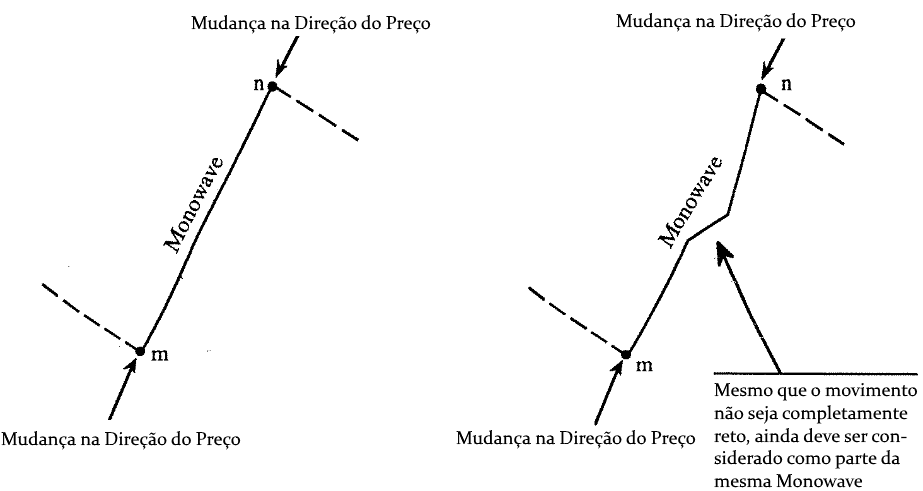
\includegraphics[width=0.8\textwidth]{NeelyMonowave.png}
	\caption{Visualização de uma Monowave}\label{fig:NeelyMonowave}
\end{figure}

Utilizando a visualização intermediária das \textbf{monowaves}, Neely criou um algoritmo
que combina \textbf{monowaves} em conjuntos que representam as Ondas de Elliott. Além disso,
o algoritmo também recombina os conjuntos identificados entre si formando Ondas de grau
superior (como listados na Tabela \ref{tab:ElliottWaveDegreeNotations}), e aplica conjuntos
de regras chamadas ``Extensões de Neely'' que, segundo Neely, estendem a capacidade de
identificação dos padrões de Elliott. Um fluxograma do algoritmo criado por Neely pode ser
visto na Figura \ref{fig:Elliott-NeelyMethod}. Como o algoritmo ainda está em estudo, no
momento só foram implementadas as funcionalidades relacionadas aos `Conceitos Gerais' e
o início da `Análise Preliminar'.

\begin{figure}[H]
	\centering
	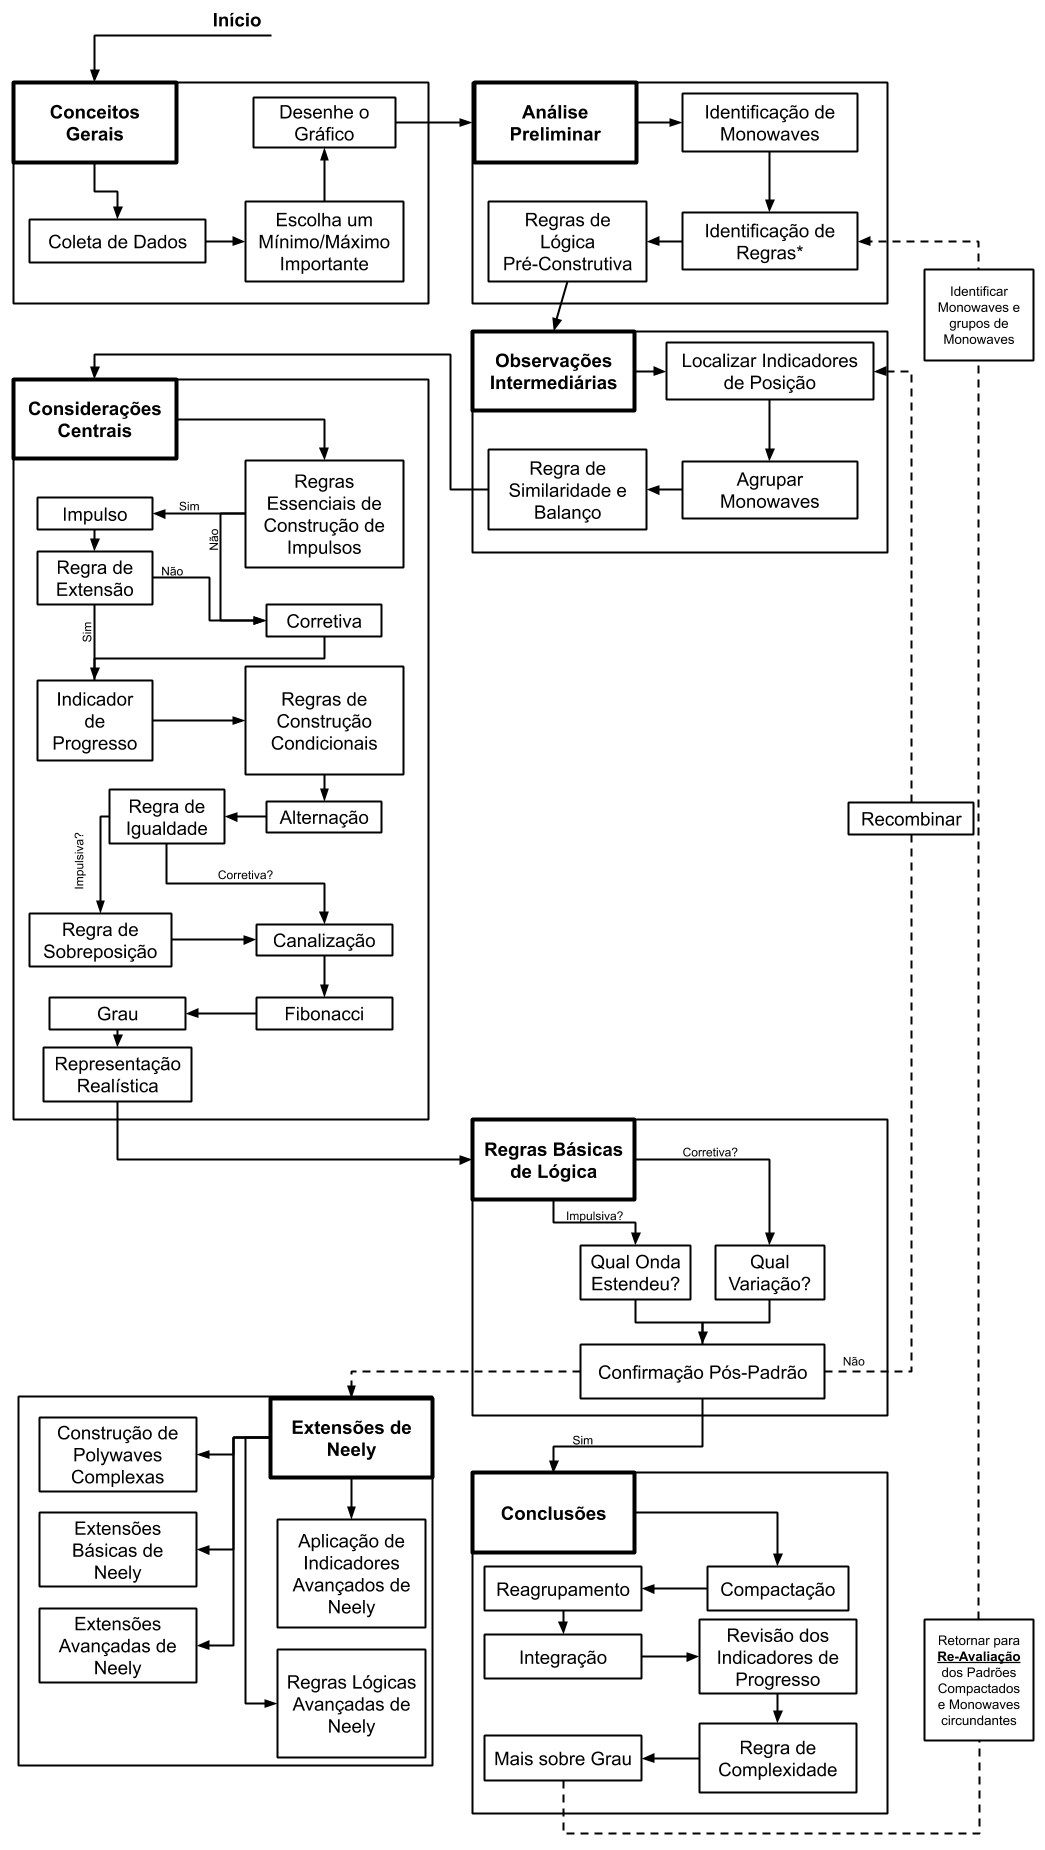
\includegraphics[width=0.8\textwidth]{Elliott-NeelyMethod.png}
	\caption{Fluxograma do Método Elliott-Neely}\label{fig:Elliott-NeelyMethod}
\end{figure}

\subsubsection{Limitação de Janela de Análise}

Na etapa da Análise Preliminar do Método Elliott-Neely, é necessário aplicar a Regra
de Neutralidade, que pode alterar o início e/ou fim das monowaves dependendo da relação entre
os pontos do gráfico e o principal Movimento Direcional.

Movimentos Direcionais são conjuntos de monowaves que movimentam o preço obrigatoriamente
para cima ou para baixo, e sua visualização pode ser vista na Figura
\ref{fig:DirectionalMovement} a seguir. Um Movimento Direcional termina quando a monowave
seguinte sofre uma retração completa, e um Movimento Direcional só se inicia quando a segunda
monowave não retrai mais do que 61,7\% da primeira.

\begin{figure}[H]
	\centering
	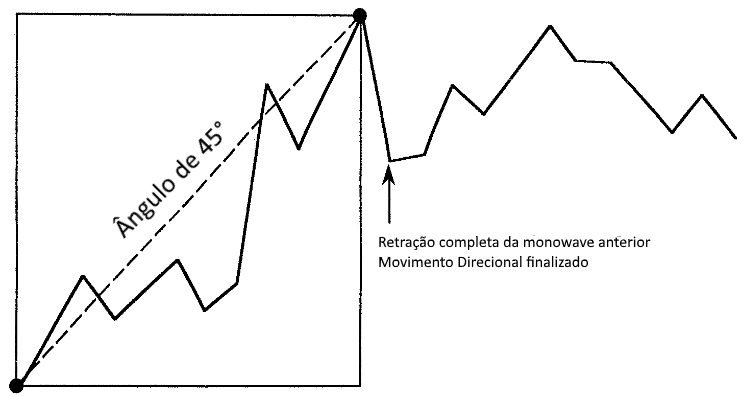
\includegraphics[width=0.8\textwidth]{DirectionalMovement.png}
	\caption{Movimento Direcional}\label{fig:DirectionalMovement}
\end{figure}

A Regra da Neutralidade consiste em identificar movimentos horizontais do preço,
e alterar os inícios e/ou fim das monowaves próximas ao movimento horizontal. Estes movimentos
horizontais podem ser vistos na Figura \ref{fig:HorizontalPriceMovement} a seguir.

\begin{figure}[H]
	\centering
	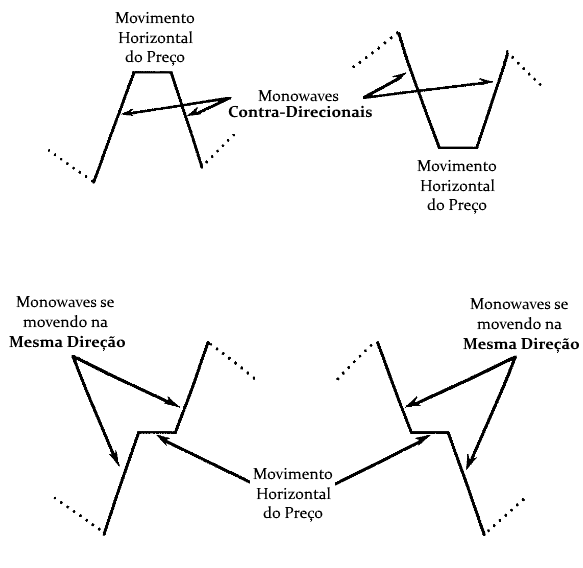
\includegraphics[width=0.7\textwidth]{HorizontalPriceMovement.png}
	\caption{Movimento Horizontal do Preço}\label{fig:HorizontalPriceMovement}
\end{figure}

A Regra de Neutralidade não se aplica se o movimento horizontal tiver ângulo maior que
\ang{45}, o que implica que as monowaves mantém seus inícios e fins originais. Quando o
movimento horizontal do preço não possuir um ângulo maior do que \ang{45}, a Regra de
Neutralidade se aplica. Para movimentos contra-direcionais, o fim da monowave anterior ao 
movimento horizontal pode ser alterado para o fim do movimento horizontal. Para movimentos
com a mesma direção, a monowave onde está o movimento horizontal pode ser separada em 3
monowaves distintas (a parte da monowave antes do movimento horizontal, a monowave com o
movimento horizontal, e o restante da monowave). Essas regras podem ser visualizadas nas
Figuras \ref{fig:RuleOfNeutralityCheck} e \ref{fig:RuleOfNeutralityExecution} a seguir.

\begin{figure}[H]
	\centering
	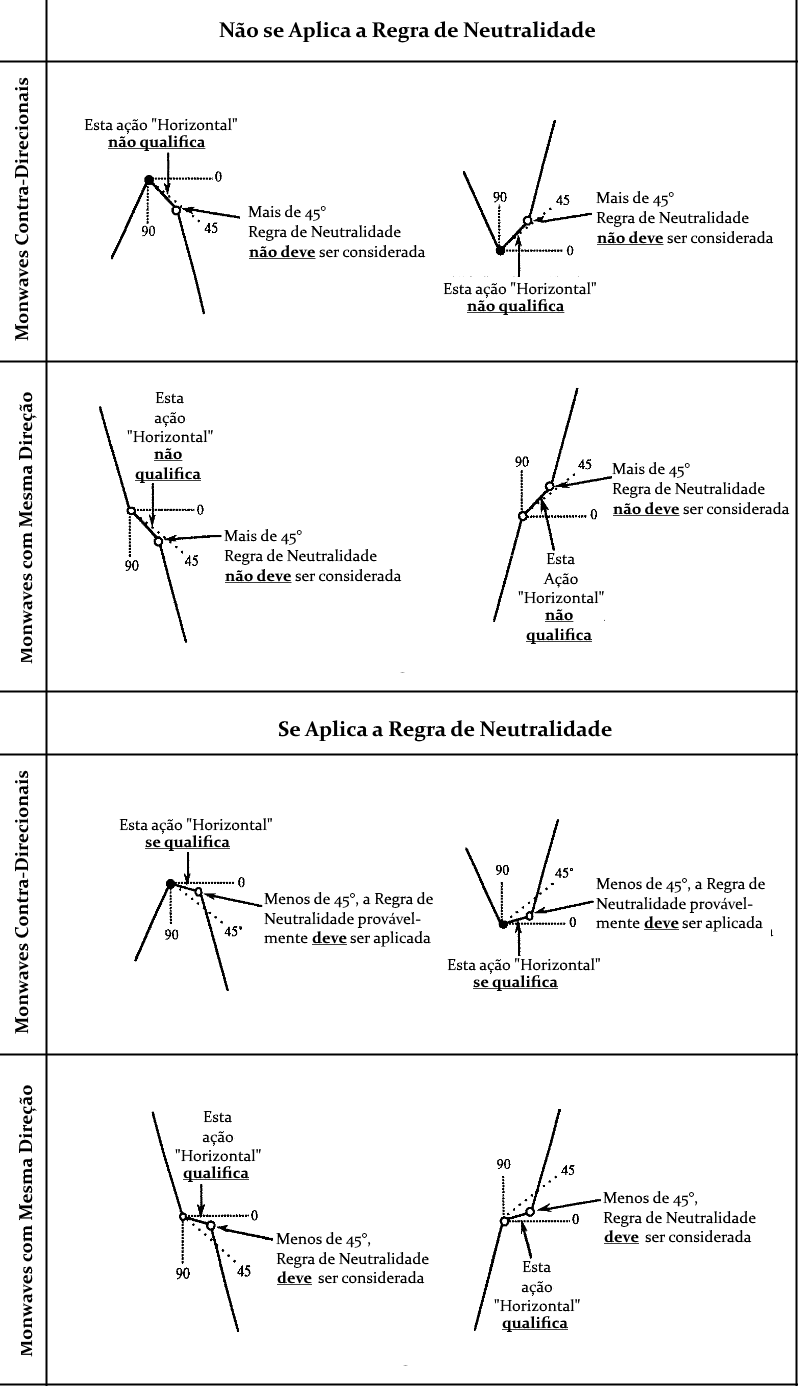
\includegraphics[width=0.7\textwidth]{RuleOfNeutralityCheck.png}
	\caption{Regra de Neutralidade em forma gráfica}\label{fig:RuleOfNeutralityCheck}
\end{figure}

\begin{figure}[H]
	\centering
	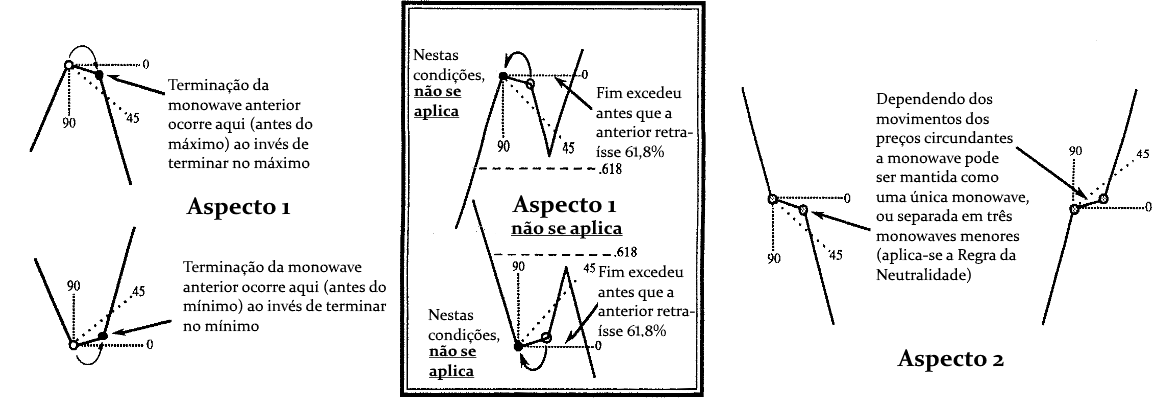
\includegraphics[width=\textwidth]{RuleOfNeutralityExecution.png}
	\caption{Execução da Regra de Neutralidade em forma gráfica}
	\label{fig:RuleOfNeutralityExecution}
\end{figure}

Na aplicação da Regra de Neutralidade, o primeiro Movimento Direcional dita quais monowaves
devem ter seu início ou fim alterado de acordo com as regras descritas anteriormente,
já que o primeiro Movimento Direcional deve alterar a escala de tempo de forma que o
primeiro Movimento Direcional possua um ângulo de \ang{45}.
Porém, Neely diz que o primeiro Movimento Direcional dita a Regra de Neutralidade para
todos os pontos de análise do gráfico, e que o gráfico ideal a ser analisado tem um total
de cerca de 30 pontos de análise em um papel de 8 polegadas.

Visto que a implementação deste algoritmo em computador não possui a limitação física (tamanho
do papel), a Regra de Neutralidade será modificada para atualizar o Movimento Direcional
usado para julgar as monowaves a cada novo Movimento Direcional que ocorrer. Dessa forma,
todas as monowaves serão julgadas pelo Movimento Direcional que ocorreu imediatamente
anterior a elas.

\subsubsection{Fatores de Estudo} \label{sec:AnalysisConfigurations}

As Extensões de Neely não especificam algumas configurações que podem alterar a
análise resultante. O preço a ser utilizado é definido por Neely como sendo o de Negociação
(\textit{Cash Market}). Neely cita que Mercados de Negociação costumam gerar uma única cotação
por dia, e essa cotação deve ser usada para compor as análises. Porém, Neely também cita
que alguns Mercados de Negociação operam continuamente, e que nesses casos, uma opção é
escolher um período de tempo para a análise, e usar a média entre o máximo e mínimo do período.

Uma ressalva feita por Neely é de que mercados internacionais devem ser observados somente
durante o período em que o mercado está aberto no país onde se está fazendo a negociação.

\begin{itemize}
	\item Preço da Ação
	\begin{itemize}
		\item Média Agregada (HLC)
		\item Mediana (HL)
		\item Preço de Fechamento (C)
	\end{itemize}
	\item Atualização da Regra de Neutralidade
	\begin{itemize}
		\item Atualiza fator a cada novo Movimento Direcional
		\item Não atualizar fator
		\item Não usar Regra de Neutralidade
	\end{itemize}
	\item Escala de Tempo
	\begin{itemize}
		\item Todas as escalas devem usar mesma configuração?
		\item Escalas diferentes usam configurações diferentes?
	\end{itemize}
\end{itemize}

Após a finalização do algoritmo, serão feitas análises de ações com diferentes configurações,
e serão observadas as diferenças nos resultados obitidos para cada configuração.
O objetivo destes testes será analisar o efeito e impacto de cada configuração sobre a
análise resultante.

\newpage

\section{Arquitetura}

Nesta seção será descrita a arquitetura do programa que implementa o algoritmo estudado.

\subsection{Contexto do Sistema}

Um programa capaz de implementar a classificação das Ondas de Elliott de forma consistente
e replicável pode se tornar uma forte ferramenta na análise de variações de preços de ativos
no mercado financeiro. A característica programática das Extensões de Neely tornam o método
de Elliott-Neely um ótimo candidato para elaboração de um sistema de análise das
variações de preços de ativos no mercado financeiro.

\subsection{Requisitos}

Nesta seção são delineados os requisitos para o sistema a ser implementado.
Inicialmente, a visão arquitetural e as partes interessadas são apresentadas, seguidas dos
requisitos de alto nível e casos de uso. Finalmente, os requisitos funcionais,
não-funcionais e evolutivos são apresentados.

\subsubsection{Visão arquitetural}

Nesta parte os principais conceitos arquiteturais serão destacados e explicados.

A entrada utilizada no sistema são os preços de \textbf{ativos}, explicados na Seção
\ref{sec:OHLC}. O sistema em desenvolvimento neste projeto de pesquisa
atualmente utiliza os dados exportados de outros softwares
em um arquivo .CSV (\textit{comma separated values}).
Há planos de configurar o programa para obter os dados atualizados em tempo real, assim
permitindo uma análise dinâmica. A implementação atual, estática através de um arquivo
.CSV, foi escolhida por ser mais simples de se implementar, além de reduzir a dependência
de programas de terceiros.

A \textbf{interface gráfica} é a parte da aplicação através da qual o usuário final interage
com o sistema e acessa suas funcionalidades.

O \textbf{algoritmo Elliott-Neely} é a parte crítica do sistema, sendo o principal responsável
pela análise dos preços de ativos alimentados no sistema. O algoritmo é discutido na Seção
\ref{sec:Neely-Extensions} e sua implementação programática é o objeto de estudo deste
Mestrado.

O \textbf{relatório final} é o resultado da análise fornecida pelo sistema. Ele será
implementado na forma gráfica, em notações de Elliott explicadas na Seção
\ref{sec:Elliott-Waves}. Caso a conclusão do algoritmo seja antecipada ao cronograma,
será implementada e emissão de um relatório escrito.

\subsubsection{\textit{Stakeholders}}

O \textbf{usuário final} é o pesquisador/analisador de mercado interessado em realizar uma
análise das Ondas de Elliott nos preços de um ativo do mercado financeiro. Seus interesses são
obter um resultado confiável dos dados analisados e conseguir utilizar o sistema sem grandes
dificuldades.

O \textbf{desenvolvedor} é um pesquisador/programador interessado em atualizar e/ou modificar
o sistema, podendo por exemplo, adicionar novos métodos de análise. Seus interesses são a
manutenibilidade do sistema e a testabilidade do sistema e de seus elementos.

Para determinação dos atributos chaves de qualidade do sistema em desenvolvimento neste
projeto de pesquisa, foi utilizado um sistema de pontuação onde cada \textit{stakeholder}
é igualmente importante e recebe 100 pontos para distribuir entre os atributos de qualidade
que ele considera importantes.
A Tabela \ref{tab:stakeholders} mostra a distribuição dos interesses de cada 
\textit{stakeholder}, assim como o interesse total de cada atributo do sistema.

\begingroup
\renewcommand*{\arraystretch}{2}
\begin{table}[H]
	\centering
	\caption{Representação Quantitativa dos Interesses dos \textit{Stakeholders}}
	\label{tab:stakeholders}
	\begin{tabular}{ L{4cm} | C{1cm} C{1cm} C{1cm} C{1cm} }
		\textbf{Stakeholders} & 
		\rotatebox{90}{\textbf{Confiabilidade}\hspace{2pt}} &
		\rotatebox{90}{\textbf{Manutenibilidade}\hspace{2pt}} &
		\rotatebox{90}{\textbf{Usabilidade}\hspace{2pt}} &
		\rotatebox{90}{\textbf{Testabilidade}\hspace{2pt}} \\
		\hline
		\textbf{Usuário Final}	&  80 &     &  20 &     \\
		\textbf{Desenvolvedor}	&  30 &  40 &     &  30 \\
		\hline
		\textbf{Total}			& 110 &  40 &  20 &  30 \\
	\end{tabular}	
\end{table}
\endgroup

\subsubsection{Atributos de Qualidade}

Os atributos chaves de qualidade são aqueles que concentram o maior interesse dos
\textit{stakeholders} (Tabela \ref{tab:stakeholders}).

\textbf{Confiabilidade} é o atributo chave deste sistema. Por ser um sistema de análise de dados,
a confiabilidade dos resultados está diretamente ligada a qualidade do sistema em si.

\textbf{Manutenibilidade} é um atributo secundário deste sistema. A medida que novos
pesquisadores se interessem no sistema, a facilidade de extensão, otimização e manutenção
se toram chaves em manter o interesse dos novos desenvolvedores.

\textbf{Testabilidade} permitirá que desenvolvedores tenham mais confiança a cerca do sistema
e das modificações feitas nele.

\textbf{Usabilidade} facilitará a interação dos usuários com o sistema.

\subsubsection{Requisitos de Alto-Nível}

Os seguintes requisitos representam as funcionalidades de alto-nível do sistema.
Cada requerimento de alto-nível será refinado em detalhe por vários requisitos específicos
e técnicos.

\begingroup
\renewcommand*{\arraystretch}{1.5}

\centering

\begin{tabular}{|p{1cm} p{2cm} p{9cm}|}
	\hline
	\multicolumn{3}{|l|}{\textbf{Análise de Dados}}\\
	HL-1 & Obrigatório & O sistema deve permitir a importação dos dados de análise.\\
	\hline
\end{tabular}

\begin{tabular}{|p{1cm} p{2cm} p{9cm}|}
	\hline
	\multicolumn{3}{|l|}{\textbf{Análise de Dados}}\\
	HL-2 & Obrigatório & O sistema deve fazer uma análise das Ondas de Elliott de acordo com as
						 Extensões de Neely de forma precisa e confiável.\\
	\hline
\end{tabular}

\begin{tabular}{|p{1cm} p{2cm} p{9cm}|}
	\hline
	\multicolumn{3}{|l|}{\textbf{Configuração da Análise}}\\
	HL-3 & Obrigatório & O sistema deve exibir os resultados da análise de forma legível para
						 o usuário.\\
	\hline
\end{tabular}

\begin{tabular}{|p{1cm} p{2cm} p{9cm}|}
	\hline
	\multicolumn{3}{|l|}{\textbf{Exibição de Resultados}}\\
	HL-4 & Obrigatório & O sistema deve permitir a mudança da configuração da análise a ser
						 feita sobre os dados.\\
	\hline
\end{tabular}

\endgroup

\subsubsection{Casos de Uso}\label{sec:UseCases}

O diagrama de casos de uso é ilustrado na Figura \ref{fig:UseCaseDiagram}, demonstrando os mais
importantes casos de uso e seus atores.

\begin{figure}[H]
	\centering
	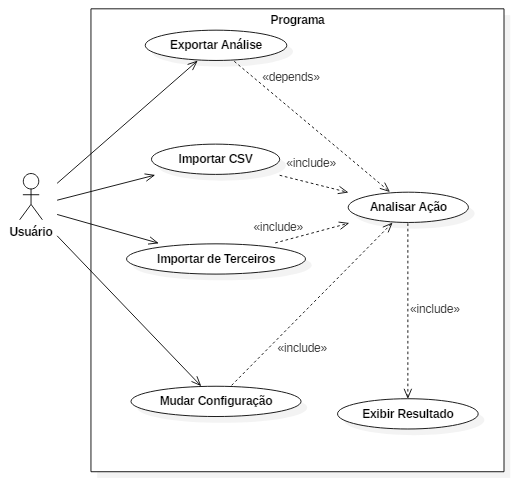
\includegraphics[width=0.8\textwidth]{UseCaseDiagram.png}
	\caption{Diagrama de Casos de Uso}\label{fig:UseCaseDiagram}
\end{figure}

Além disso, as Tabelas a seguir mostram os casos de uso arquiteturalmente significantes.
A numeração refere-se ao requerimento de Alto-nível, por exemplo, UC-1.x refere-se a HL-1.

\begingroup
\renewcommand*{\arraystretch}{1.2}
\begin{table}[H]
	\caption{UC-1.1 - Importar .CSV}
	\label{tab:UC-1.1}
	\begin{tabular}{p{6cm} p{8cm}}
		\multicolumn{2}{l}{\large{\textbf{UC-1.1 - Importar .CSV}}}\\
		\toprule
		\textbf{Ator Primário}		&	Usuário Final \\
		\midrule
		\textbf{Objetivo}			&	Importar um Arquivo .CSV com preços de ativo a serem analisados \\
		\midrule
		\textbf{Condições Iniciais}	&	O sistema está operacional, e o usuário final possui
										o arquivo com o histórico da Ação a ser analisada \\
		\midrule
		\textbf{Cenário Principal de Sucesso}	& \\
		& \begin{enumerate}
			\item O usuário clica na opção de Inserir o Arquivo .CSV com os dados da Ação
			\item O usuário localiza o arquivo .CSV a ser analisado
			\item O sistema valida o arquivo .CSV
			\item O sistema realiza a análise do histórico de preços da Ação (UC-2.1)
		\end{enumerate}\\
		\midrule
		\textbf{Extensões}	& \\
		& \begin{enumerate}
			\item[3.a] O sistema identifica que o arquivo .CSV não tem as colunas necessárias
			\begin{enumerate}
				\item[3.a.1] O sistema não analisa o arquivo .CSV
				\item[3.a.2] O sistema emite um aviso de que o arquivo .CSV não é válido
				\item[3.a.3] O usuário obtém um arquivo .CSV válido
				\item[3.a.4] Ir para o passo 1 
			\end{enumerate}
		\end{enumerate}\\
		\midrule
		\textbf{Sub-variações} & \\
		& \\
		\midrule
		\textbf{Condições Finais} & O histórico de preços da ação é analisado e o usuário final
									pode alterar as configurações de análise. \\
		\midrule
		\textbf{Requisitos Relacionados} & HL-1, FR-1, FR-2 \\
		\bottomrule
	\end{tabular}		
\end{table}

\begin{table}[H]
	\caption{UC-1.2 - Importar de Terceiros}
	\label{tab:ImportFromThirdParty}
	\begin{tabular}{p{6cm} p{8cm}}
		\multicolumn{2}{l}{\large{\textbf{UC-1.2 - Importar de Terceiros}}}\\
		\toprule
		\textbf{Ator Primário}		&	Usuário Final \\
		\midrule
		\textbf{Objetivo}			&	Importar os preços de ativo a serem analisados via terceiros\\
		\midrule
		\textbf{Condições Iniciais}	&	O sistema está operacional, e o usuário final possui
										uma fonte de dados alternativa \\
		\midrule
		\textbf{Cenário Principal de Sucesso}	& \\
		& \begin{enumerate}
			\item O usuário configura o programa  para estabelecer a conexão com o terceiro
			\item O sistema valida as configurações da conexão com o terceiro
			\item O sistema requisita os dados do terceiro
			\item O sistema realiza a análise do histórico de preços da Ação (UC-2.1)
		\end{enumerate}\\
		\midrule
		\textbf{Extensões}	& \\
		& \begin{enumerate}
			\item[2.a] O sistema não consegue realizar a conexão com o terceiro
			\begin{enumerate}
				\item[2.a.1] O sistema não realiza a análise
				\item[2.a.2] O sistema emite um aviso de que a conexão não foi estabelecida
				\item[2.a.3] Ir para o passo 1 
			\end{enumerate}
		\end{enumerate}\\
		\midrule
		\textbf{Sub-variações} & \\
		& \\
		\midrule
		\textbf{Condições Finais} & O histórico de preços da ação é analisado e o usuário final
									pode alterar as configurações de análise. \\
		\midrule
		\textbf{Requisitos Relacionados} & HL-1, FR-6 \\
		\bottomrule
	\end{tabular}		
\end{table}

\begin{table}[H]
	\caption{UC-2.1 - Analisar Ação}
	\label{tab:UC-2.1}
	\begin{tabular}{p{6cm} p{8cm}}
		\multicolumn{2}{l}{\large{\textbf{UC-2.1 - Analisar Ação}}}\\
		\toprule
		\textbf{Ator Primário}		&	Sistema \\
		\midrule
		\textbf{Objetivo}			&	Analisar o Histórico de Preços de uma Ação \\
		\midrule
		\textbf{Condições Iniciais}	&	O sistema está operacional, e o arquivo foi inserido
										pelo usuário e validado pelo sistema\\
		\midrule
		\textbf{Cenário Principal de Sucesso}	& \\
		& \begin{enumerate}
			\item O sistema realiza a análise do histórico de preços da Ação.
			\item O sistema exibe os resultados para o usuário (UC-3.1)
		\end{enumerate}\\
		\midrule
		\textbf{Extensões}	& \\
		& \\
		\midrule
		\textbf{Sub-variações} & \\
		& \\
		\midrule
		\textbf{Condições Finais} & A interface exibe o resultado da análise e o usuário
									pode alterar as configurações de análise. \\
		\midrule
		\textbf{Requisitos Relacionados} & HL-2, FR-3 \\
		\bottomrule
	\end{tabular}		
\end{table}

\begin{table}[H]
	\caption{UC-3.1 - Exibir Resultado}
	\label{tab:UC-3.1}
	\begin{tabular}{p{6cm} p{8cm}}
		\multicolumn{2}{l}{\large{\textbf{UC-3.1 - Exibir Resultado}}}\\
		\toprule
		\textbf{Ator Primário}		&	Sistema \\
		\midrule
		\textbf{Objetivo}			&	Exibir o resultado da análise feita \\
		\midrule
		\textbf{Condições Iniciais}	&	O sistema finalizou uma análise (UC-2.1) \\
		\midrule
		\textbf{Cenário Principal de Sucesso}	& \\
		& \begin{enumerate}
			\item O sistema deve exibir o gráfico do histórico do preço da Ação
			\item O sistema deve sobrepor a este gráfico as notações das Ondas de Elliott
		\end{enumerate}\\
		\midrule
		\textbf{Extensões}	& \\
		& \\
		\midrule
		\textbf{Sub-variações} & \\
		& \\
		\midrule
		\textbf{Condições Finais} & O resultado da análise é visível para o usuário final. \\
		\midrule
		\textbf{Requisitos Relacionados} & HL-3, FR-4 \\
		\bottomrule
	\end{tabular}		
\end{table}

\begin{table}[H]
	\caption{UC-4.1 - Mudar Configuração}
	\label{tab:UC-4.1}
	\begin{tabular}{p{6cm} p{8cm}}
		\multicolumn{2}{l}{\large{\textbf{UC-4.1 - Mudar Configuração}}}\\
		\toprule
		\textbf{Ator Primário}		&	Usuário Final \\
		\midrule
		\textbf{Objetivo}			&	Alterar as configurações de análise \\
		\midrule
		\textbf{Condições Iniciais}	&	Um conjunto de dados já foi inicializado no sistema \\
		\midrule
		\textbf{Cenário Principal de Sucesso}	& \\
		& \begin{enumerate}
			\item O usuário altera uma das configurações disponíveis na interface
			\item O sistema atualiza a análise de acordo com as novas configurações (UC-2.1)
		\end{enumerate}\\
		\midrule
		\textbf{Extensões}	& \\
		& \\
		\midrule
		\textbf{Sub-variações} & \\
		& \\
		\midrule
		\textbf{Condições Finais} & A análise é atualizada para a nova configuração. \\
		\midrule
		\textbf{Requisitos Relacionados} & HL-4, FR-3, FR-4, FR-5\\
		\bottomrule
	\end{tabular}		
\end{table}

\endgroup

O Caso de Uso UC-1.2 descrito na Tabela \ref{tab:ImportFromThirdParty} que importa dados
de terceiros é uma funcionalidade planejada. O objetivo é que os dados sejam obtidos,
por exemplo, diretamente através de uma interface TCP/IP, ou através de uma conexão com
um programa como o MetaTrader 5. Se esta funcionalidade for implementada, a atualização
dos dados e da análise poderá ser feita em tempo real, a medida que novos dados sejam
disponibilizados.

\subsubsection{Requisitos Funcionais}

Nesta seção, os requisitos que capturam o comportamento esperado do sistema serão
apresentados (Tabela \ref{tab:functional-requirements}). Este comportamento pode ser
expresso como serviços, tarefas ou funções que o sistema deve executar.
Estes são derivados a partir dos requisitos de Alto-nível e dos casos de uso.

\begingroup
\renewcommand*{\arraystretch}{1.2}
\begin{table}[H]
	\centering
	\caption{Requisitos Funcionais}
	\label{tab:functional-requirements}
	\begin{tabular}{p{1cm} p{2cm} p{10cm}}
		FR-1 & Obrigatório & O sistema deve validar se a entrada é válida.\\
		\midrule
		FR-2 & Obrigatório & O sistema deve informar o usuário caso a entrada seja inválida.\\
		\midrule
		FR-3 & Obrigatório & O sistema deve realizar a análise automaticamente.\\
		\midrule
		FR-4 & Obrigatório & O sistema deve exibir o resultado ao usuário automaticamente.\\
		\midrule
		FR-5 & Obrigatório & O sistema deve atualizar automaticamente a análise quando o
							 usuário alterar as configurações.\\
		\midrule
		FR-6 & Desejável   & E desejável que o sistema consiga obter os dados através de uma 
							 conexão com um terceiro.\\
	\end{tabular}		
\end{table}
\endgroup

\subsection{Análise}

Esta seção foca em esclarecer o processo de desenvolvimento do sistema. Aqui, todas as
suposições que são relevantes ao processo são mostradas, assim como o roteiro tecnológico de
desenvolvimento e as decisões de alto-nível tomadas durante o projeto.

\subsubsection{Suposições}

\begin{itemize}
	\item O usuário final tem conhecimento sobre o mercado de ações (Seção \ref{sec:Stockmarket});
	\item O usuário final tem conhecimento sobre a representação dos preços de ações (Seção \ref{sec:OHLC});
	\item O usuário final tem conhecimento sobre as Ondas de Elliott (Seção \ref{sec:Elliott-Waves});
	\item O usuário final tem a sua disposição um software capaz de exportar os preços da
		  ação que quer analisar em formato .CSV;
\end{itemize}

\subsubsection{Roteiro tecnológico}

A primeira versão do sistema foi desenvolvida somente para gerar a representação gráfica
do histórico de preços e implementar mudanças de configurações básicas. Esta versão teve
como objetivo demonstrar que o ambiente de desenvolvimento era favorável e compatível
com a aplicação a ser criada.

A segunda versão do sistema está sendo desenvolvida para implementar a análise de preços
de ações no mercado financeiro conforme o método de Elliott-Neely. Esta versão será capaz
de realizar uma análise das Ondas de Elliott de forma automática, com mínima ou nenhuma
intervenção do usuário.

Versões futuras do sistema serão capazes de realizarem previsões futuras dos preços das
ações a partir, primariamente, da verificação dos padrões das Ondas de Elliott.

\subsection{Arquitetura do Software}

A arquitetura do software é descrita nesta seção. Esta seção é composta dos principais
motivadores arquiteturais, seguidos das visões arquiteturais. A representação foi criada
baseada no modelo 4+1 \cite{Kruchten:1995}, \emph{i.e.}, consistindo na visão lógica,
visão de processo, visão de desenvolvimento, visão física e visão de caso de uso.
Para fortalecer o conceito original do modelo 4+1, cada visão foi projetada usando
UML \cite{UML}, conforme recomendado em \cite{FCG:2007}.

\subsubsection{Visão Lógica}

Esta visão mostra as abstrações chaves e mecanismos que são usados dentro do programa
para realizar suas funcionalidades. A interação entre estes elementos também é descrita.
Os elementos estão alocados em camadas de acordo com suas responsabilidades. A representação 
gráfica desta visão pode ser observada na Figura \ref{fig:LogicView}. Foi utilizado o
padrão MVC para esta Visão \cite{KrasnerPope:1988} \cite{Buschmann:1988}.

\begin{figure}[H]
	\centering
	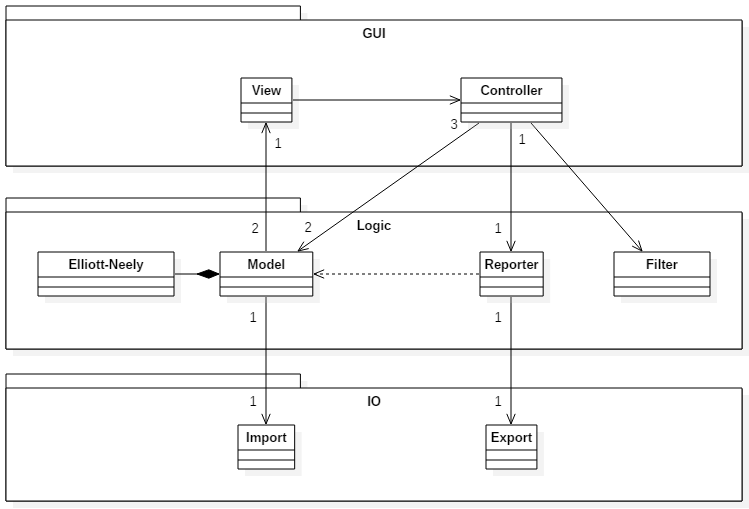
\includegraphics[width=\textwidth]{LogicView.png}
	\caption{Visão Lógica}\label{fig:LogicView}
\end{figure}

\begin{itemize}
	\item \textbf{GUI}: Interface com Usuário
	\begin{itemize}
		\item A \textbf{Visualização} (\textbf{\textit{View}}) é a parte da camada de interface com a qual o usuário interage diretamente, acessando as funcionalidades do programa.
		\item O \textbf{Controlador} (\textbf{\textit{Controller}}) são os dispositivos lógicos e de controle que realizam as funcionalidades do programa. O programa utiliza 3 controladores: Global (para funcionalidades gerais), Data (para processamento de dados) e UI (para interfaceamento gráfico).
	\end{itemize}
	\item \textbf{Logic}: Lógica
	\begin{itemize}
		\item O \textbf{Modelo} (\textbf{\textit{Model}}) é a parte da camada lógica onde se encontram os dados sendo processados pelo programa ou visualizados na interface. Estão sendo utilizados dois Modelos: um de dados (sob o qual o Método de \textbf{Elliott-Neely} é aplicado), e um de visualização, que é enviado para a \textbf{GUI}.
		\item O \textbf{Relator} (\textbf{\textit{Reporter}}) é a parte responsável por criar uma relatório para o usuário.
		\item O \textbf{Filtro} (\textbf{\textit{Filter}}) é responsável por filtrar quais informações serão disponibilizadas para o usuário de acordo com a configuração escolhida.
	\end{itemize}
	\item \textbf{IO}: Entradas e Saídas
	\begin{itemize}
		\item A \textbf{Importação} (\textbf{\textit{Import}}) é responsável por receber os dados do usuário.
		\item A \textbf{Exportação} (\textbf{\textit{Export}}) é responsável por enviar dados para o usuário.
	\end{itemize}
\end{itemize}


\subsubsection{Visão de Processo}

Esta visão mostra a representação abstrata do processo principal no sistema. Para apresentar
estas representações, os casos de uso descritos na Seção \ref{sec:UseCases} foram utilizados
para retratar as partes envolvidas na realização de cada caso de uso.

\begin{figure}[H]
	\centering
	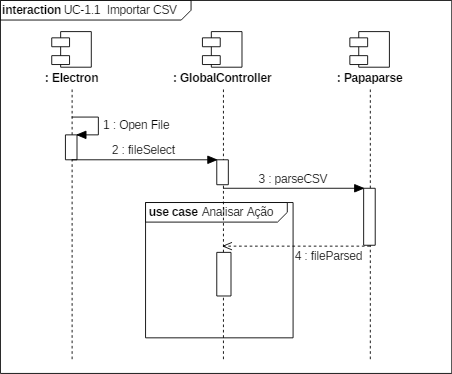
\includegraphics[width=0.7\textwidth]{ProcessViewUC-1_1.png}
	\caption{Visão de Processo para \hyperref[tab:UC-1.1]{UC-1.1: Importar CSV}}
	\label{fig:ProcessView-UC-1.1}
\end{figure}

\begin{figure}[H]
	\centering
	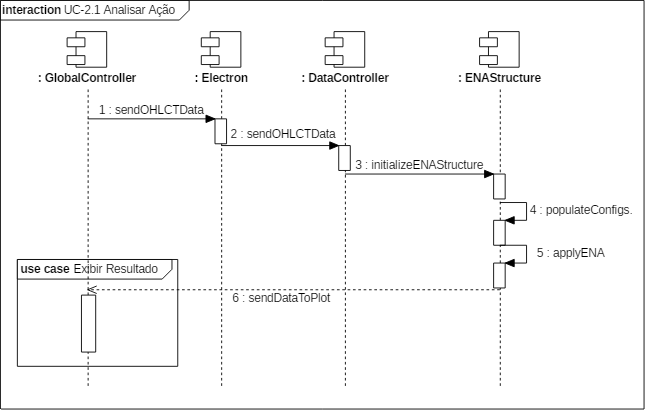
\includegraphics[width=\textwidth]{ProcessViewUC-2_1.png}
	\caption{Visão de Processo para \hyperref[tab:UC-2.1]{UC-2.1: Analisar Ação}}
	\label{fig:ProcessView-UC-2.1}
\end{figure}

\begin{figure}[H]
	\centering
	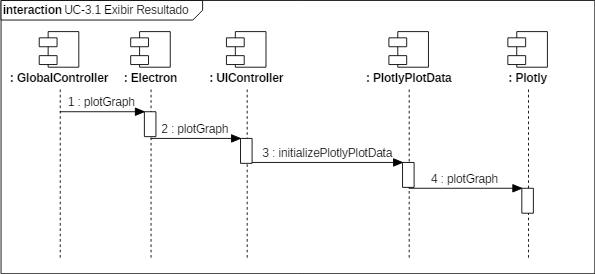
\includegraphics[width=\textwidth]{ProcessViewUC-3_1.png}
	\caption{Visão de Processo para \hyperref[tab:UC-3.1]{UC-3.1: Exibir Resultado}}
	\label{fig:ProcessView-UC-3.1}
\end{figure}

\begin{figure}[H]
	\centering
	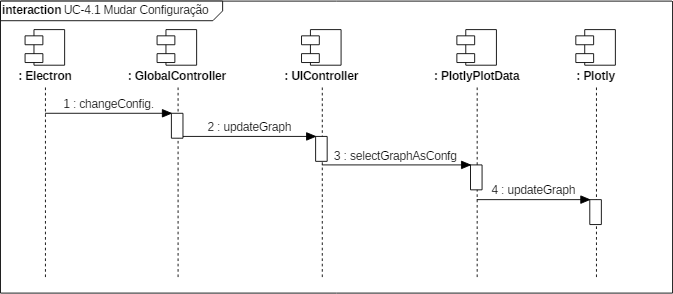
\includegraphics[width=\textwidth]{ProcessViewUC-4_1.png}
	\caption{Visão de Processo para \hyperref[tab:UC-4.1]{UC-4.1: Mudar Configuração}}
	\label{fig:ProcessView-UC-4.1}
\end{figure}

\subsubsection{Visão de Implementação}

Essa visão foca no gerenciamento de configuração e organização real do módulo de software
no ambiente de desenvolvimento, englobando os principais componentes usados para montar e
gerar o sistema físico. Nas seções a seguir, esses componentes são decompostos e descritos
em termos de responsabilidades e interfaces.
A representação gráfica desta visão pode ser observada na Figura \ref{fig:DevelopmentView}.

\begin{figure}[H]
	\centering
	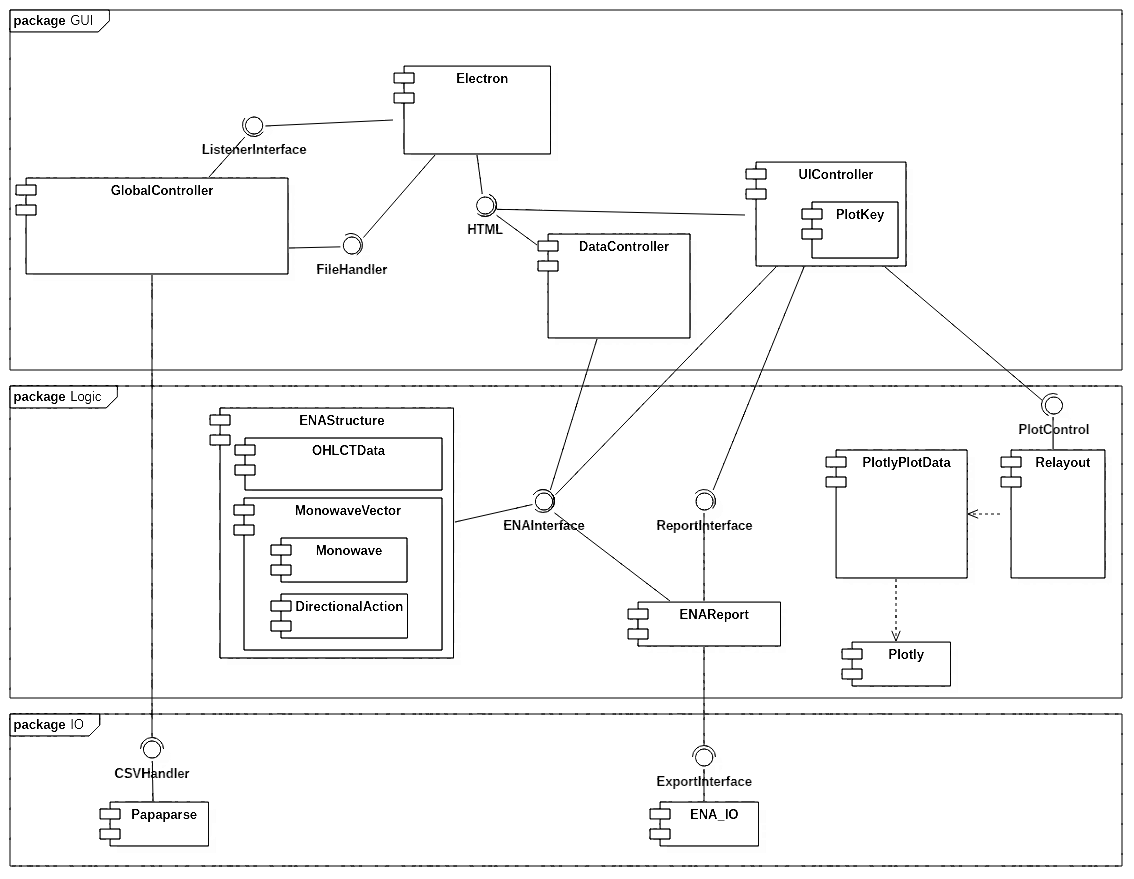
\includegraphics[width=\textwidth]{DevelopmentView.png}
	\caption{Visão de Implementação}\label{fig:DevelopmentView}
\end{figure}

Foi usado um padrão de 3 Módulos para implementação do sistema. Cada módulo age como um
controlador de responsabilidades específicas.
O Controlador de Dados (\textit{DataController}) gerencia os dados da aplicação: 
neste caso, o modelo de dados estudados (o \textbf{\textit{ENAStructure}}).
O Controlador de UI gerencia a parte de interface visual com o usuário: plota o gráfico
(utilizando a biblioteca Plotly \cite{Plotly}).
O Controlador Global (\textit{GlobalController}) gerencia os outros Controladores,
eventos (\textit{e.g.} clique em botão, seleção de opção, entrada de arquivo), e faz
a conversão do arquivo .CSV em um objeto JavaScript (usando a biblioteca
PapaParse \cite{PapaParse}).

\begin{itemize}
	\item \textbf{Electron}
	\begin{itemize}
		\item É o framework usado no desenvolvimento, e o programa onde a aplicação do sistema executa.
		\item Ele implementa as interfaces com usuário através de HTML e CSS, funcionalidades de controle através dos observadores de evento (\textit{ListenerInterface}), e importa os dados através da interface \textit{FileHandler}.
	\end{itemize}
	\item \textbf{GlobalController}
	\begin{itemize}
		\item Controlador geral da aplicação.
		\item Responsabilidades:
		\begin{itemize}
			\item Implementar e gerenciar eventos (\textit{e.g.} clique em botão, seleção de opção, entrada de arquivo) via \textbf{Electron} usando a interface \textbf{ListenerHTML}.
			\item Receber os dados de entrada do usuário a partir da interface \textbf{FileHandler}.
			\item Converter o arquivo .CSV do usuário usando a biblioteca \textbf{Papaparse} via interface \textbf{CSVHandler}.
			\item Gerenciar os outros Controladores por meio do \textbf{Electron}.
		\end{itemize}
	\end{itemize}
	\item \textbf{DataController}
	\begin{itemize}
		\item Gerenciador dos dados da aplicação.
		\item Responsabilidades:
		\begin{itemize}
			\item Receber os dados entrados pelo usuário via interface \textbf{HTML}.
			\item Salvar os dados entrados pelo usuário no modelo \textbf{ENAStructure} via interface \textbf{ENAInterface}.
		\end{itemize}
	\end{itemize}
	\item \textbf{UIController}
	\begin{itemize}
		\item Gerenciador da visualização e interface com usuário.
		\item Possui uma estrutura chamada \textbf{PlotKey} que registra as modificações feitas nas configurações de exibição quando o programa solicitar uma atualização do gráfico.
		\item Responsabilidades:
		\begin{itemize}
			\item Receber os dados para plotar o gráfico via interface \textbf{ENAInterface}.
			\item Plotar o gráfico usando a biblioteca \textbf{Plotly} via interface \textbf{PlotControl}.
			\item Enviar os dados para geração do relatório da análise para o componente \textbf{ENAReport} via interface \textbf{ReportInterface}.
		\end{itemize}
	\end{itemize}
	\item \textbf{ENAStructure}
	\begin{itemize}
		\item Organiza os dados do usuário de acordo com as configurações possíveis.
		\item Os dados do usuário são salvos na estrutura \textbf{OHLCTStructure}.
		\item A análise gerada é feita e salva na estrutura \textbf{MonowaveVector}.
		\item A estrutura \textbf{MonowaveVector} realiza a análise através da organização de um vetor de \textbf{Monowave}(s) e de uma estrutura de \textbf{DirectionalAction}.
		\item Para cada combinação de configurações disponíveis, são gerados um par de \textbf{OHLCTData} e \textbf{MonowaveVector}
	\end{itemize}
	\item \textbf{ENAReport}
	\begin{itemize}
		\item Gera um relatório da análise para o usuário.
		\item O relatório gerado é exportado para o usuário através do módulo \textbf{ENA\_IO} via interface \textbf{ExportInterface}.
	\end{itemize}
	\item \textbf{Relayout}
	\begin{itemize}
		\item Guarda o histórico de visualizações do gráfico, permitindo desfazer e refazer comandos de Zoom.
		\item Permite aplicar um comando de Fit vertical para melhor utilizar o espaço horizontal do gráfico.
	\end{itemize}
	\item \textbf{PlotlyPlotData}
	\begin{itemize}
		\item Guarda os dados da \textbf{ENAStructure} formatados para visualização usando a biblioteca \textbf{Plotly}.
	\end{itemize}
\end{itemize}

\subsubsection{Visão de Implantação}

Esta visão foca na distribuição do software no hardware. Ela apresenta o hardware e as
peças de software que o compõem. A seguir, cada parte do software e hardware serão explicadas.
A representação gráfica desta visão pode ser observada na Figura \ref{fig:DeploymentView}.

\begin{figure}[H]
	\centering
	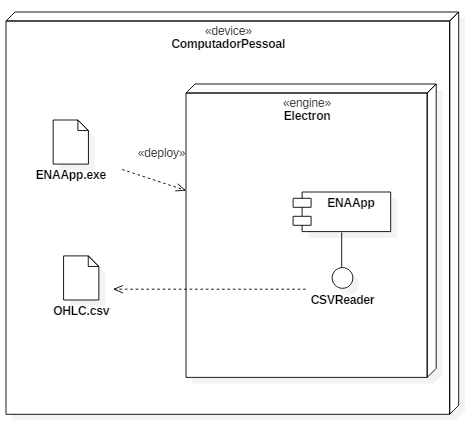
\includegraphics[width=0.7\textwidth]{DeploymentView.png}
	\caption{Visão de Implantação}\label{fig:DeploymentView}
\end{figure}

O \textbf{computador pessoal} representa qualquer computador pessoal rodando um sistema
operacional Windows, Linux ou MacOS.

O \textbf{ENAApp.exe} é o arquivo executável gerado a partir do projeto. Ele está listado
como ``.exe'' a título de exemplo e simplificação, pois o Electron é capaz de gerar programas
para vários sistemas operacionais utilizando o mesmo código fonte.

O executável cria uma instância do \textbf{Electron}, na qual a aplicação ``Elliott-Neely 
Analysis App'' (\textbf{ENAApp}) executa. A aplicação é capaz de importar arquivos .csv
através da interface \textbf{CSVReader}. Na visualização, o arquivo OHLC.csv é usado como
exemplo.

\subsubsection{Decisões de Desenvolvimento de Software}

Esta seção lista as decisões relacionadas ao desenvolvimento do software e implementação.
Elas podem ser vistas nas Tabelas seguintes. O modelo utilizado para estas decisões foi
baseado em \cite{TyreeAckerman:2005}.

\begingroup
\renewcommand*{\arraystretch}{1.2}

\begin{table}[H]
	\centering
	\caption{Decisão - Linguagem de Implementação}
	\begin{tabular}{p{3cm} p{11cm}}
		\textbf{Nome}		&	Linguagem de Implementação \\
		\toprule
		\textbf{Decisão}	&   \\
							& 1 \\
		\toprule
		\midrule
		\textbf{Estado}		& Aprovada \\
		\midrule
		\textbf{Problema}	& Qual linguagem de programação utilizar para implementar o algoritmo\\
		\midrule
		\textbf{Decisão}	& Electron (\textit{framework}) + JavaScript (lógica)
							  + HTML5 \& CSS (interface)\\
		\midrule
		\textbf{Alternativas} & \\
		& \textit{C}, \textit{Java}, \textit{C\#}, \textit{Ruby}, \textit{Python} \\
		\midrule
		\textbf{Argumentos} & \\
		& JavaScript é uma linguagem interpretada, com interpretadores disponíveis em vários
		  sistemas operacionais, muitos destes possuindo código aberto com licenças permissivas
		  (como o Chrome V8 \cite{ChromeV8}).\\
		& Node.js \cite{Node.js} é um \textit{runtime} para JavaScript que implementa uma
		  modificação da \textit{engine} Chrome V8, permitindo a execução de código em JavaScript
		  sem a necessidade de um navegador web.\\
		& NPM \cite{NPM} é um catálogo de bibliotecas e projetos em JavaScript, reunindo mais
		  de 60 mil módulos e controle de versão para cada módulo.\\
		& Electron \cite{ElectronJS} é um \textit{framework} que permite a criação de programas
		  em JavaScript + HTML5 \& CSS capazes de rodar em diversos sistemas operacionais 
		  sem problemas de compatibilidade.\\
		& JavaScript possui tipificação dinâmica de variáveis, o que permite uma maior
		  flexibilidade na criação e manuseio de dados.\\
		& Este ecossistema permite a criação de aplicações altamente flexíveis e compatíveis,
		  com acesso a um grande acervo de bibliotecas e módulos para serem integrados,
		  sem problemas de licenciamento e com controle de versão individual por módulo.\\
		\bottomrule
	\end{tabular}		
\end{table}

\begin{table}[H]
	\centering
	\caption{Decisão - Análise de Diferentes Configurações}
	\begin{tabular}{p{3cm} p{11cm}}
		\textbf{Nome}		&	Análise de Diferentes Configurações \\
		\toprule
		\textbf{Decisão}	&   \\
							& 2 \\
		\toprule
		\midrule
		\textbf{Estado}		& Aprovada \\
		\midrule
		\textbf{Problema}	& Como fazer a análise para as diferentes configurações, conforme listadas e descritas na Seção \ref{sec:AnalysisConfigurations}\\
		\midrule
		\textbf{Decisão}	& Fazer a análise para todas as configurações possíveis e somente alterar qual está visível\\
		\midrule
		\textbf{Alternativas} & \\
		& \begin{enumerate}
			\item Realizar a análise somente para a configuração atual e refazer a análise para cada mudança na configuração
			\item Registrar cada análise feita e somente refazer a análise caso uma nova configuração seja escolhida
			\item Fazer a análise para todas as configurações possíveis e somente alterar qual está visível
		\end{enumerate} \\
		\midrule
		\textbf{Argumentos} & \\
		& A opção 1 implica em um menor gasto inicial de recursos, já que seria feita somente uma análise, mas causaria desperdício de recursos quando fosse solicitada a análise de uma configuração já visualizada anteriormente. \\
		& A opção 2 levaria implicaria na necessidade de se implementar um controle adicional para verificar se a análise já foi feita antes. \\
		& A opção 3 implica em um maior gasto inicial de recursos e facilita a mudança entre configurações. \\
		& Visto que a implementação deste sistema visa a exploração das diferentes configurações, foi decido pela terceira opção. \\
		\bottomrule
	\end{tabular}		
\end{table}

\endgroup


\newpage

\section{Cronograma e Progressão}

Nesta seção são listadas as atividades previstas para realização do trabalho proposto.
Na Tabela \ref{tab:cronograma} é apresentado o cronograma para estas atividades.
Na Tabela \ref{tab:progresso} são listadas as atividades individuais envolvidas na elaboração
e programação do algoritmo estudado.

\begin{enumerate}
	\item Obtenção dos créditos referentes as disciplinas do Mestrado;
	\item Pesquisa bibliográfica;
	\item Redação da monografia para o Exame Geral de Qualificação;
	\item Exame Geral de Qualificação;
	\item Elaboração do algoritmo proposto e programação;
	\item Geração e execução de casos de testes, e avaliação do sistema;
	\item Análise dos efeitos das configurações sobre os resultados do algoritmo;
	\item Redação final da Dissertação; e
	\item Defesa do Mestrado.
\end{enumerate}

\begingroup
\newcommand{\y}{\rule{13,2pt}{5pt}}
\newcommand{\x}{\hspace*{2pt}}
\setlength{\tabcolsep}{0pt}
\begin{table}[H]
	\footnotesize
	\centering
	\begin{tabular}{|l|c|c|c|c|c|c|c|c|c|c|c|c|c|c|c|c|c|c|c|c|c|c|c|c|}
  	\cline{2-25}
  	\multicolumn{1}{l|}{} & \multicolumn{5}{c|}{2018} & \multicolumn{12}{c|}{2019} & \multicolumn{7}{c|}{2020}\\
  	\cline{2-25}
  	\multicolumn{1}{c|}{\textbf{Atividades}} &
	\rotatebox{90}{Agosto\hspace{2pt}} &
	\rotatebox{90}{Setembro\hspace{2pt}} &
	\rotatebox{90}{Outubro\hspace{2pt}} &
	\rotatebox{90}{Novembro\hspace{2pt}} &
	\rotatebox{90}{Dezembro\hspace{2pt}} &
	\rotatebox{90}{Janeiro\hspace{2pt}} &
	\rotatebox{90}{Fevereiro\hspace{2pt}} &
	\rotatebox{90}{Março\hspace{2pt}} &
	\rotatebox{90}{Abril\hspace{2pt}} &
	\rotatebox{90}{Maio\hspace{2pt}} &
	\rotatebox{90}{Junho\hspace{2pt}} &
	\rotatebox{90}{Julho\hspace{2pt}} &
	\rotatebox{90}{Agosto\hspace{2pt}} &
	\rotatebox{90}{Setembro\hspace{2pt}} &
	\rotatebox{90}{Outubro\hspace{2pt}} &
	\rotatebox{90}{Novembro\hspace{2pt}} &
	\rotatebox{90}{Dezembro\hspace{2pt}} &
	\rotatebox{90}{Janeiro\hspace{2pt}} &
	\rotatebox{90}{Fevereiro\hspace{2pt}} &
	\rotatebox{90}{Março\hspace{2pt}} &
	\rotatebox{90}{Abril\hspace{2pt}} &
	\rotatebox{90}{Maio\hspace{2pt}} &
	\rotatebox{90}{Junho\hspace{2pt}} &
	\rotatebox{90}{Julho\hspace{2pt}} \\
	\hline 

	1. Créditos					& \y & \y & \y & \y & \y & \y & \y & \y & \y & \y & \y & \y & \x & \x & \x & \x & \x & \x & \x & \x & \x & \x & \x & \x\\ \hline
	2. Pesquisa bibliográfica	& \y & \y & \y & \y & \y & \y & \y & \y & \y & \y & \y & \y & \y & \y & \y & \y & \y & \y & \y & \y & \y & \y & \y & \x\\ \hline
	3. Escrita da qualificação	& \x & \x & \x & \x & \x & \x & \x & \x & \x & \x & \y & \y & \y & \x & \x & \x & \x & \x & \x & \x & \x & \x & \x & \x\\ \hline
	4. Exame de qualificação	& \x & \x & \x & \x & \x & \x & \x & \x & \x & \x & \x & \x & \x & \y & \x & \x & \x & \x & \x & \x & \x & \x & \x & \x\\ \hline
	5. Elaboração do prog.		& \y & \y & \y & \y & \y & \y & \y & \y & \y & \y & \x & \x & \y & \y & \y & \y & \y & \y & \x & \x & \x & \x & \x & \x\\ \hline
	6. Testes					& \x & \x & \x & \x & \x & \x & \x & \x & \x & \x & \x & \x & \x & \x & \x & \x & \y & \y & \x & \x & \x & \x & \x & \x\\ \hline
	7. Análise de config.		& \x & \x & \x & \x & \x & \x & \x & \x & \x & \x & \x & \x & \x & \x & \x & \x & \x & \x & \y & \y & \y & \x & \x & \x\\ \hline
	8. Escrita da dissertação	& \x & \x & \x & \x & \x & \x & \x & \x & \x & \x & \x & \x & \x & \x & \x & \x & \x & \x & \x & \x & \x & \y & \y & \y\\ \hline
	9. Defesa do mestrado		& \x & \x & \x & \x & \x & \x & \x & \x & \x & \x & \x & \x & \x & \x & \x & \x & \x & \x & \x & \x & \x & \x & \x & \y\\ \hline	
	\end{tabular}
\caption{Cronograma de atividades}
\label{tab:cronograma}
\end{table}
\endgroup

\newpage

\begingroup
\renewcommand*{\arraystretch}{1.5}
\begin{table}[H]
\centering
\scriptsize
\begin{tabular}{|L{3cm}|L{2cm}|L{5cm}|R{1.4cm}|R{1.4cm}|}
	\hline
	\textbf{Tópico} & \textbf{Atividade} & \textbf{Descrição} & \textbf{Progresso} & \textbf{Estimado} \\
	\hline
	\hline
	\textbf{Aquisição de Dados}
		& \textbf{Importação de Dados}
		& 	Importação dos Dados OHLC em arquivos .CSV exportados a partir do Programa MetaTrader 5. \newline
			Utilizando a biblioteca \textbf{Papaparse}.
		& 100\%
		& - \\
	\hline
	\textbf{Pré-Tratamento de Dados}
		& \textbf{Passagem dos Dados para Classe OHLCT}
		& Transferência dos dados importados do MetaTrader 5 para a \textbf{Classe OHLCT}
		& 100\%
		& - \\
		\cline{2-5}
		& \textbf{Escalas de Tempo}
		&	Replica dados originais em diferentes escalas de tempo. \newline
			Implementados: 1 min, 1 hora, 1 dia. \newline
			Escalável para fácil configuração de novas escalas.
		& 100\%
		& - \\
		\cline{2-5}
		& \textbf{Valor Típico}
		&	Cálculo do Valor Típico sobre o qual a análise será feita. \newline
			Implementados: Valor Agregado (HLC), Mediana (HL). \newline
			Escalável para fácil configuração de novos valores típicos.
		& 100\%
		& - \\
	\hline
	\textbf{Método Elliott-Neely \newline Analise Preliminar \newline (1ª parte)}
		& \textbf{Regra de Neutralidade (1º passo)}
		&	Aplicação da primeira passagem da \textbf{Regra de Neutralidade}. \newline
			Implementado através das \textbf{Classes Monowave} e \textbf{Monowave Vector}.
		& 100\%
		& - \\
		\cline{2-5}
		& \textbf{Regra de Proporção \newline (Seleção da Janela de Análise)}
		&	Atualizada para ambiente digital e alta quantidade de dados. \newline
			Afeta a segunda passagem da \textbf{Regra de Neutralidade} e a \textbf{Regra de Retração}
		& 100\%
		& - \\
		\cline{2-5}
		& \textbf{Regra de Neutralidade (2º Passo)}
		& Une \textbf{monowaves} e/ou altera início/fim de \textbf{monowaves} de acordo com a \textbf{Regra de Proporção}.
		& 100\%
		& - \\
		\cline{2-5}
		& \textbf{Regra de Observação}
		& Aplicada de forma emergente através da \textbf{Classe Monowave Vector}.
		& 100\%
		& - \\
		\cline{2-5}
		& \textbf{Regra de Retração}
		& Classificação de \textbf{Monowaves}.
		& 0\%
		& 3 semanas \\
	\hline
	\textbf{Método Elliott-Neely \newline Observações Intermediárias \newline (2ª parte)}
		& \textbf{Regra de Similaridade e Balanço}
		& Indica quais \textbf{Monowaves} pertencem ao mesmo grupo/grau para efeito de agrupamento.
		& 0\%
		& 2 semanas \\
	\hline
	\textbf{Método Elliott-Neely \newline Considerações Centrais \newline (3ª parte)}
		& \textbf{Construção de Polywaves}
		& Classifica conjuntos de \textbf{Monowaves} nos padrões das \textbf{Ondas de Elliott}.
		& 0\%
		& 3-4 semanas \\
		\cline{2-5}
		& \textbf{Extensões de Neely}
		& Aplica regras de compactação que transformam grupos de \textbf{Monowaves} em \textbf{Monowaves} de grau maior.
		& 0\%
		& 3-4 semanas \\
	\hline
	\textbf{Interface com Usuário}
		& \textbf{Visualização em Gráfico}
		& Utilizando a biblioteca \textbf{Plotly.js}
		& 100\%
		& - \\
		\cline{2-5}
		& \textbf{Configurações}
		& Eixo Vertical (Log ou Linear), Eixo Horizontal (Tempo ou Sequencial), Tipo de Marcador (OHLC, Candelstick ou Nenhum), Resolução do Tempo (1 Minuto, 10 Minutos, 1 Hora, 1 Dia), Valor Típico (HLC ou HL), Monowave (Visualizar ou Esconder)
		& 100\%
		& - \\
	\hline
\end{tabular} 
\caption{Progresso do algoritmo}
\label{tab:progresso}
\end{table}
\endgroup

\newpage

% \section{Referências}
\raggedright
\bibliographystyle{unsrtnat}
\phantomsection
\addcontentsline{toc}{section}{Referências}
\bibliography{references}

\newpage

\phantomsection
\addcontentsline{toc}{section}{Apêndices}
\section*{Apêndices}
\renewcommand{\thesubsection}{\Alph{subsection}}

\subsection{Padrões das Ondas de Elliott} \label{app:EWPatterns}

\begin{figure}[H]
	\centering
	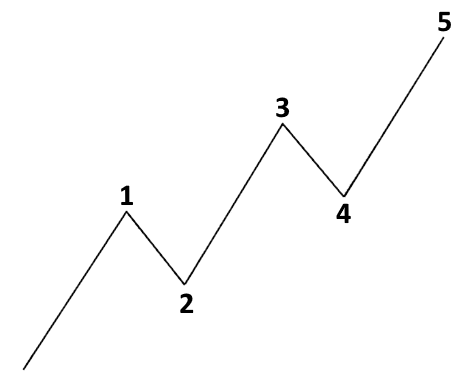
\includegraphics[width=0.7\textwidth]{EW_pattern_01.png}
	\caption{Padrão de Onda Motivadora: Impulso}\label{fig:EW_pattern_01}
\end{figure}

\begin{figure}[H]
	\centering
	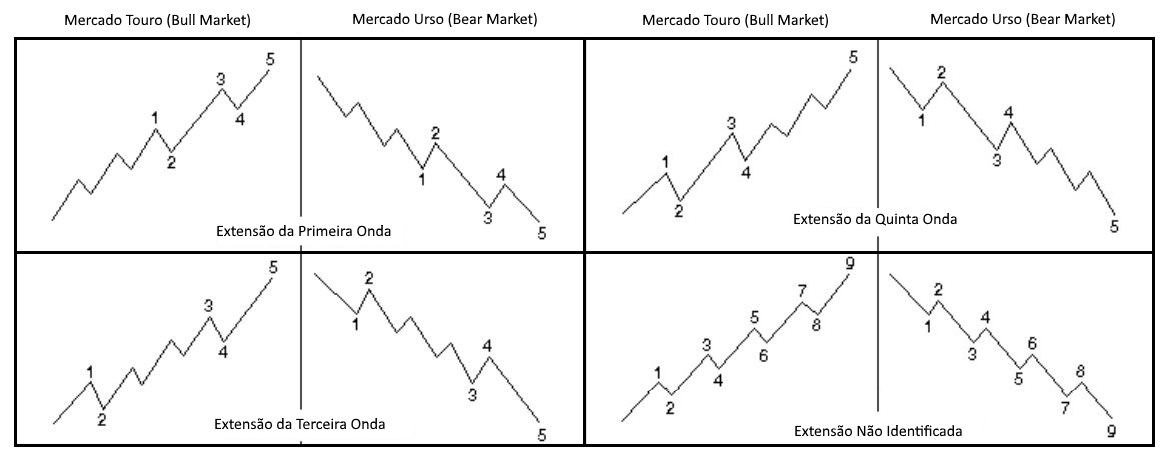
\includegraphics[width=\textwidth]{EW_pattern_02.png}
	\caption{Padrão de Onda Motivadora: Extensão}\label{fig:EW_pattern_02}
\end{figure}

\begin{figure}[H]
	\centering
	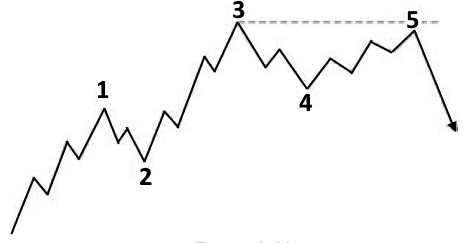
\includegraphics[width=0.7\textwidth]{EW_pattern_03.png}
	\caption{Padrão de Onda Motivadora: Truncagem}\label{fig:EW_pattern_03}
\end{figure}

\begin{figure}[H]
	\centering
	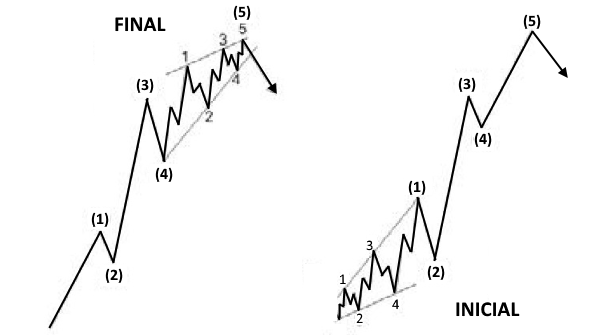
\includegraphics[width=0.7\textwidth]{EW_pattern_04.png}
	\caption{Padrão de Onda Motivadora: Diagonal Final/Inicial}\label{fig:EW_pattern_04}
\end{figure}

\begin{figure}[H]
	\centering
	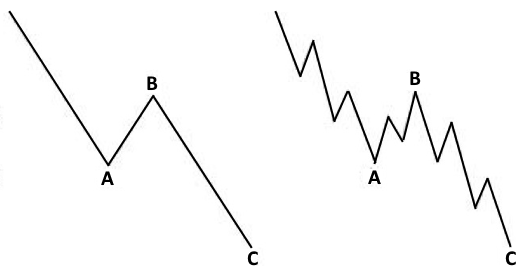
\includegraphics[width=0.7\textwidth]{EW_pattern_05.png}
	\caption{Padrão de Onda Corretiva: Zigzag}\label{fig:EW_pattern_05}
\end{figure}

\begin{figure}[H]
	\centering
	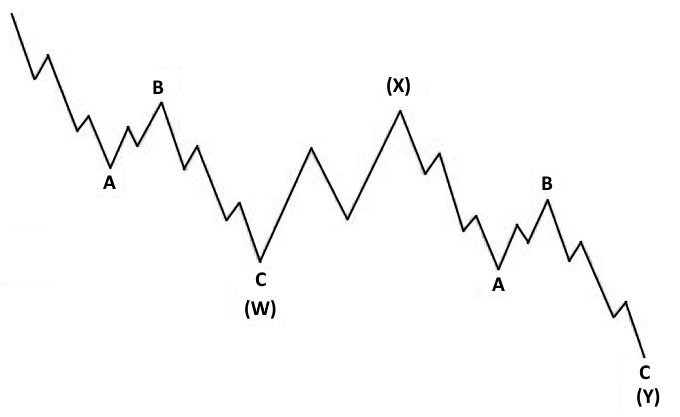
\includegraphics[width=0.7\textwidth]{EW_pattern_06.png}
	\caption{Padrão de Onda Corretiva: Zigzag Duplo}\label{fig:EW_pattern_06}
\end{figure}

\begin{figure}[H]
	\centering
	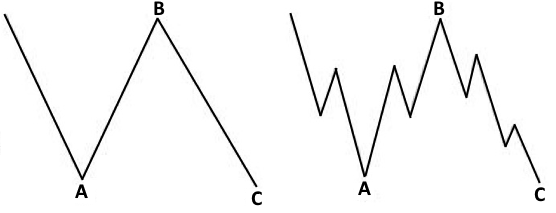
\includegraphics[width=0.7\textwidth]{EW_pattern_07.png}
	\caption{Padrão de Onda Corretiva: Plano}\label{fig:EW_pattern_07}
\end{figure}

\begin{figure}[H]
	\centering
	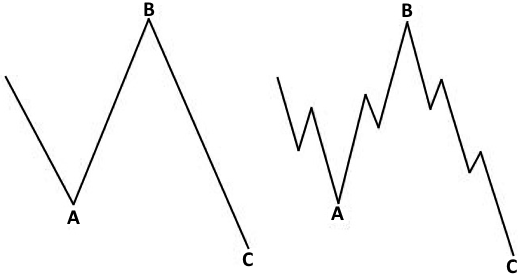
\includegraphics[width=0.7\textwidth]{EW_pattern_08.png}
	\caption{Padrão de Onda Corretiva: Plano Estendido}\label{fig:EW_pattern_08}
\end{figure}

\begin{figure}[H]
	\centering
	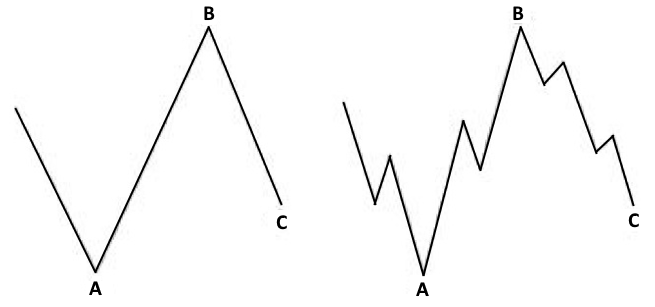
\includegraphics[width=0.7\textwidth]{EW_pattern_09.png}
	\caption{Padrão de Onda Corretiva: Plano Corrido}\label{fig:EW_pattern_09}
\end{figure}

\begin{figure}[H]
	\centering
	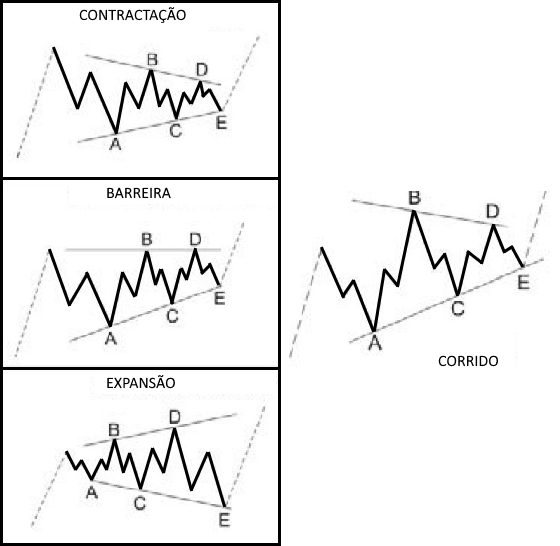
\includegraphics[width=0.7\textwidth]{EW_pattern_10.png}
	\caption{Padrão de Onda Corretiva: Triângulo}\label{fig:EW_pattern_10}
\end{figure}

\begin{figure}[H]
	\centering
	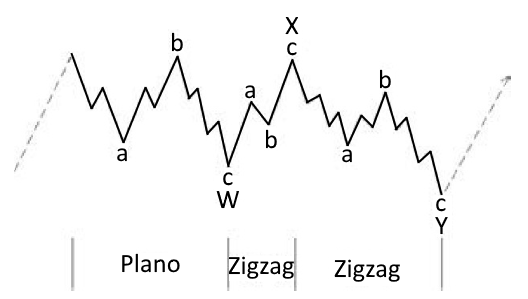
\includegraphics[width=0.7\textwidth]{EW_pattern_11.png}
	\caption{Padrão de Onda Corretiva: Combinação (exemplo 1)}\label{fig:EW_pattern_11}
\end{figure}

\begin{figure}[H]
	\centering
	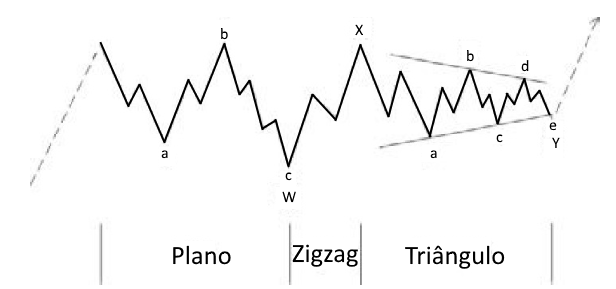
\includegraphics[width=0.7\textwidth]{EW_pattern_12.png}
	\caption{Padrão de Onda Corretiva: Combinação (exemplo 2)}\label{fig:EW_pattern_12}
\end{figure}

\end{document}
